%-----------------------
\chapter{Alkalmazás}
%-----------------------
%TODO write
%TODO spellcheck

Egy alkalmazás megvalósítása mindig komplex folyamat, mely sok kisebb részfolyamatot foglal magába. Az alábbiakban a fejlesztés részleteiről fogok írni, kezdve az alkalmazással szemben támasztott követelményekkel, majd képernyőképek segítségével bemutatom a működését. Ezután a megvalósítás részleteibe fogok belemenni, és végül a tesztelésről is ejtek pár szót.

\section{Követelmények}

A fejlesztés során alapvető célom volt egy, a modern paradigmáknak és a felhasználók elvárásainak megfelelő applikáció megalkotása. Törekedtem az objektumorientált szemlélet alkalmazására, a felelősségek szétválasztására és a maximális felhasználói élmény nyújtására. Fontos volt, hogy az alkalmazás folyamatai ne térjenek el nagymértékben attól, mint amit a felhasználók más applikációkban megszokhattak, és minden művelet meg legyen valósítva az adatokon, amire szükségük lehet.

Ezek alapján az alábbi követelmények fogalmazódtak meg az alkalmazással szemben:
\begin{enumerate}
	\item A felhasználónak legyen lehetősége fiókot létrehozni, e-mail cím és jelszó megadásával bejelentkezni, illetve fiókjából ki is lépni.
	\item Az adatok legyenek perzisztensen tárolva, az alkalmazás bezárásával, abból való kilépéssel vagy egy esetleges készülékcsere esetén se vesszenek el.
	\item Az adatok csak bejelentkezés után váljanak láthatóvá, minden felhasználó csak a saját adataihoz férhessen hozzá.
	\item A felhasználó képes legyen kategóriákat létrehozni a jegyzetek számára, ezeket akár tetszőleges mélységben további kategóriákba ágyazni.
	\item Legyen lehetőség jegyzetek létrehozására dokumentumok lefényképezése által. A szöveg digitalizálása után a jegyzet legyen címmel ellátható, kategóriába sorolható és a tartalma szerkeszthető.
	\item Inkonzisztens adatok létrehozására ne adjon lehetőséget, a felhasználói input mindig legyen validálva.
	\item A jegyzeteken és kategóriákon lehessen minden fő műveletet - létrehozás, olvasás, módosítás, törlés - elvégezni, ezek során a felhasználói felület és az adatbázis maradjanak konzisztensek egymással.
	\item Módosítás során lehessen a jegyzetet újabb fényképek készítésével kiegészíteni, az ily módon digitalizált szöveg kerüljön hozzáfűzésre az eredeti tartalomhoz.
	\item A UI esztétikai és felhasználói élmény szempontjából legyen megfelelő, a hosszú ideig tartó folyamatokat jelezze a felhasználónak töltőképernyő segítségével.
	\item A jegyzetek listája lehessen rendezhető és kereshető.
\end{enumerate}

\section{Működés}

A következőkben az alkalmazás funkcióit fogom bemutatni, a leírásokat képernyőképekkel kiegészítve. A képek néhol eltérnek egymástól, melynek oka hogy az applikáció funkcionalitásából fakadóan nem volt lehetséges mindet az emulátoron elkészíteni, hanem a jegyzetek készítéséhez fizikai készülékre is szükség volt.

\subsection{Bejelentkezés}
A telepítést követően a bejelentkezési képernyő az első, amivel a felhasználó találkozik. Ez már korábban megjelent a dolgozatban, a \refstruc{fig:MaterialBeforeAfter} bemutatásában. Itt a beviteli mezők segédszövegei egyértelműsítik, hogy milyen adatok elvártak a bejelentkezéshez illetve regisztrációhoz. Ezek gombnyomás hatására validálásra kerülnek, és amennyiben az e-mail formátuma nem érvényes vagy a jelszó hossza nem éri el a 6 karaktert, akkor a folyamat meghiúsul, és a felhasználó értesül róla, hogy mely mező(k) tartalmát kell javítania.

\subsection{Kategorizált lista}
Sikeres bejelentkezést követően az alkalmazás a fő képernyőjére navigál, ahol az eddig elmentett jegyzeteket láthatjuk kategóriákba rendezve. A kategóriák alapértelmezetten össze vannak csukva, csak a legfelső szinten található elemeket látjuk. A lista sorainak jobb szélén elhelyezkedő nyilakra kattintva tudjuk kibontani az adott kategóriát, ezzel megtekinteni a tartalmát (\refstruc{fig:NoteListScreen}).

\begin{figure}[!ht]
	\centering
	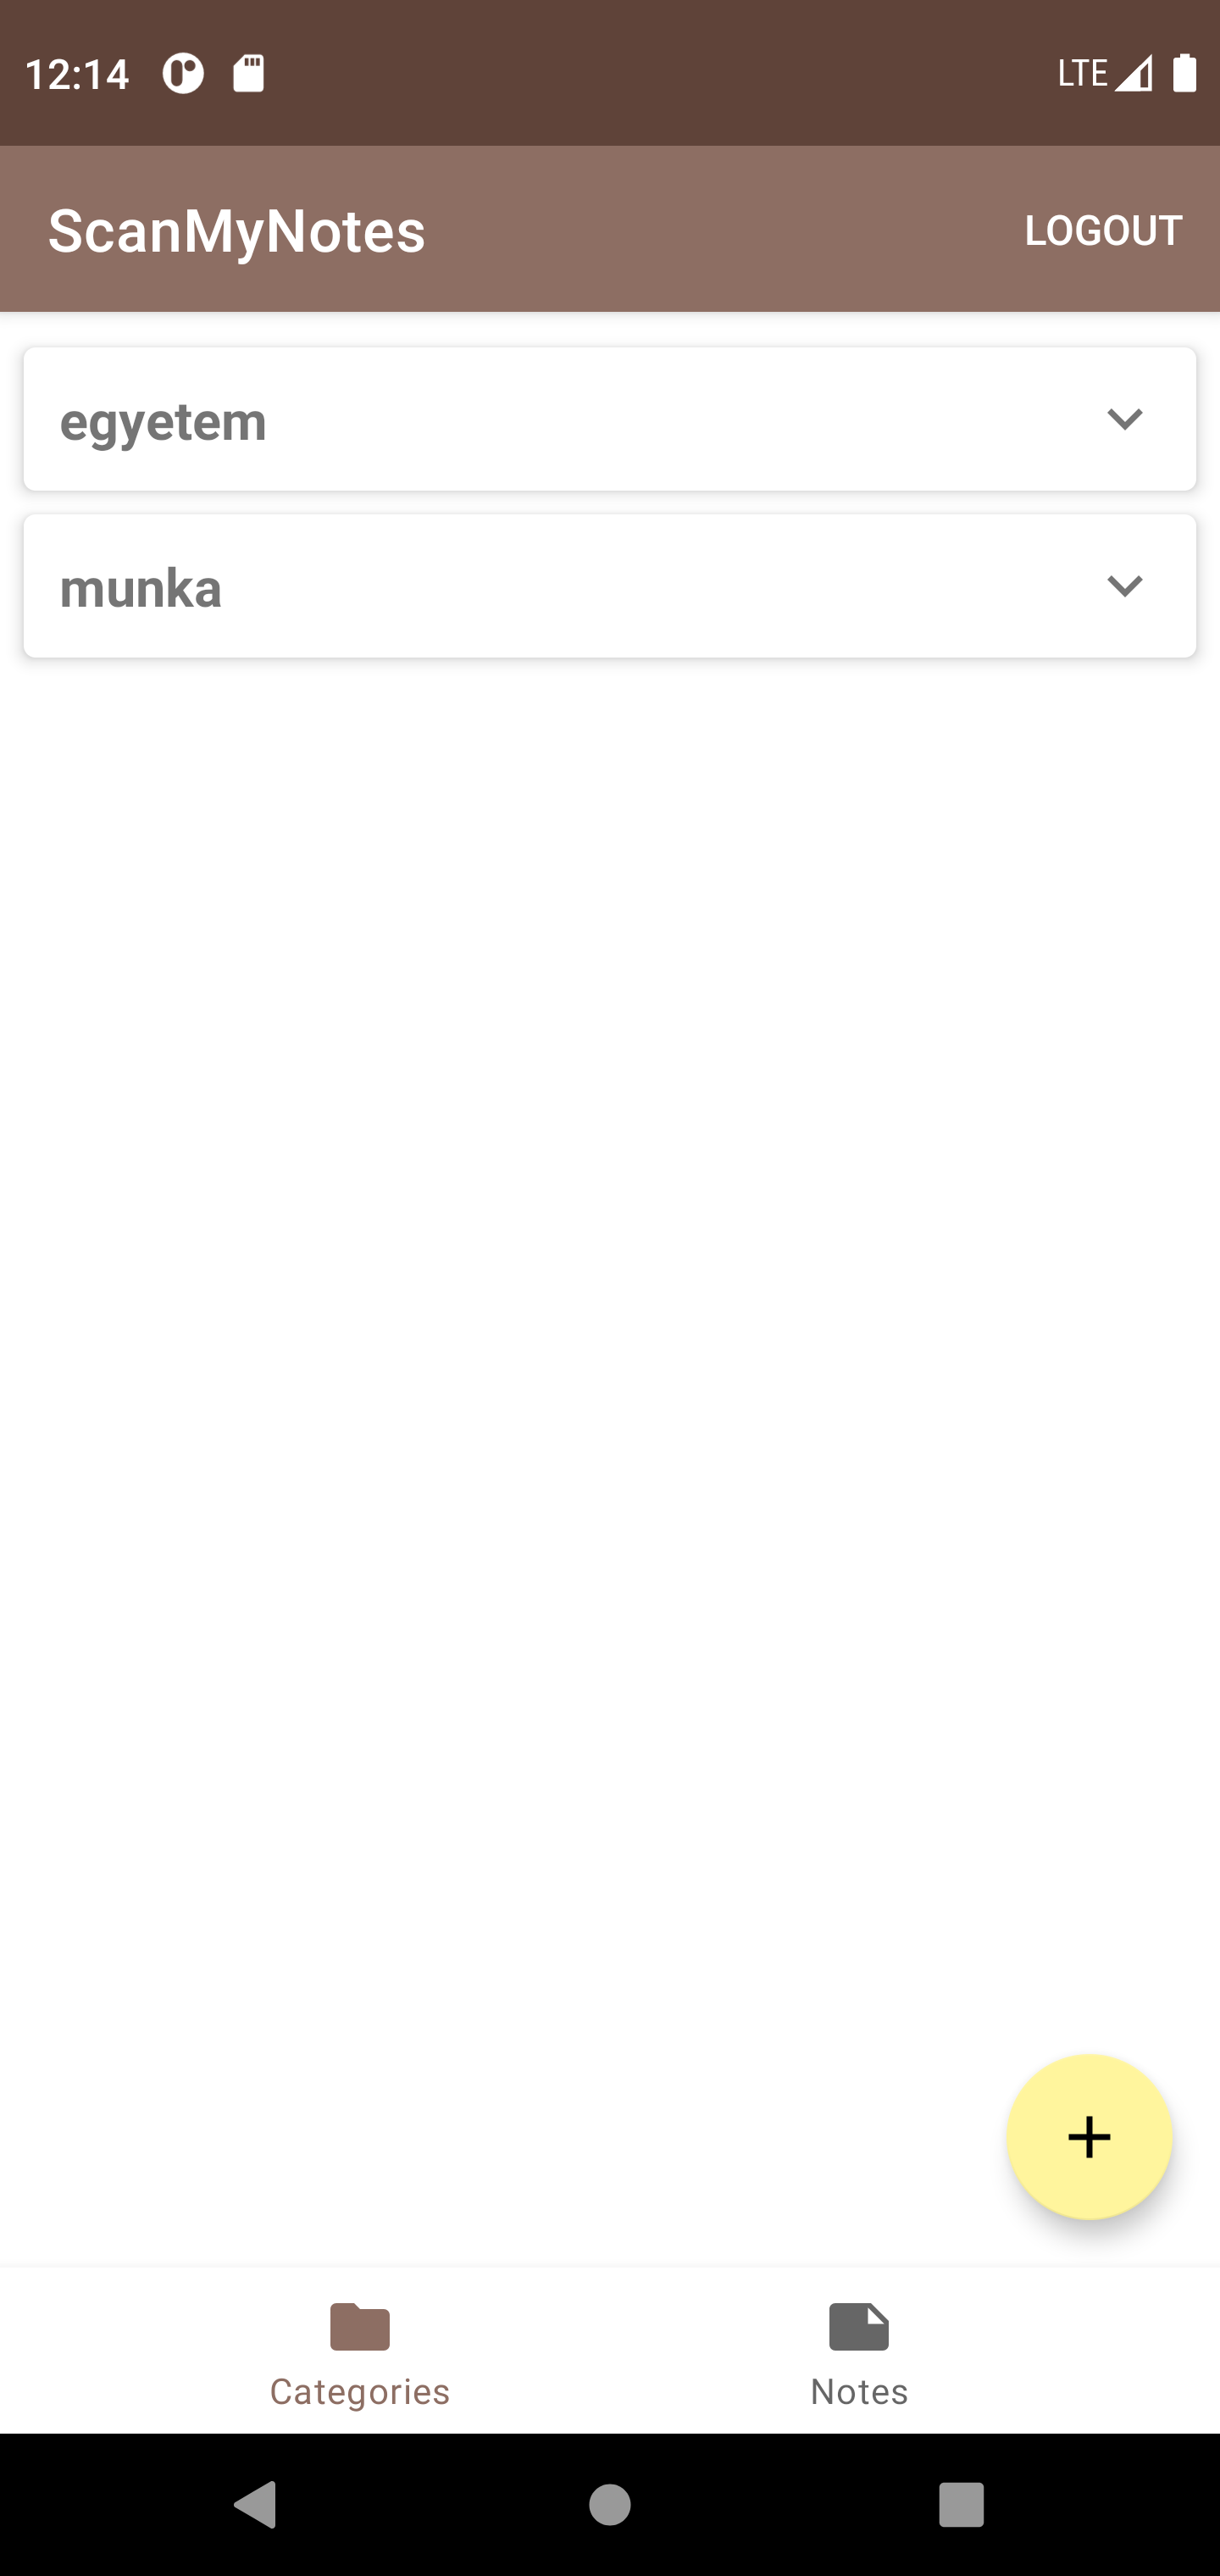
\includegraphics[width=55mm, keepaspectratio]{figures/notelist_closed.png}
	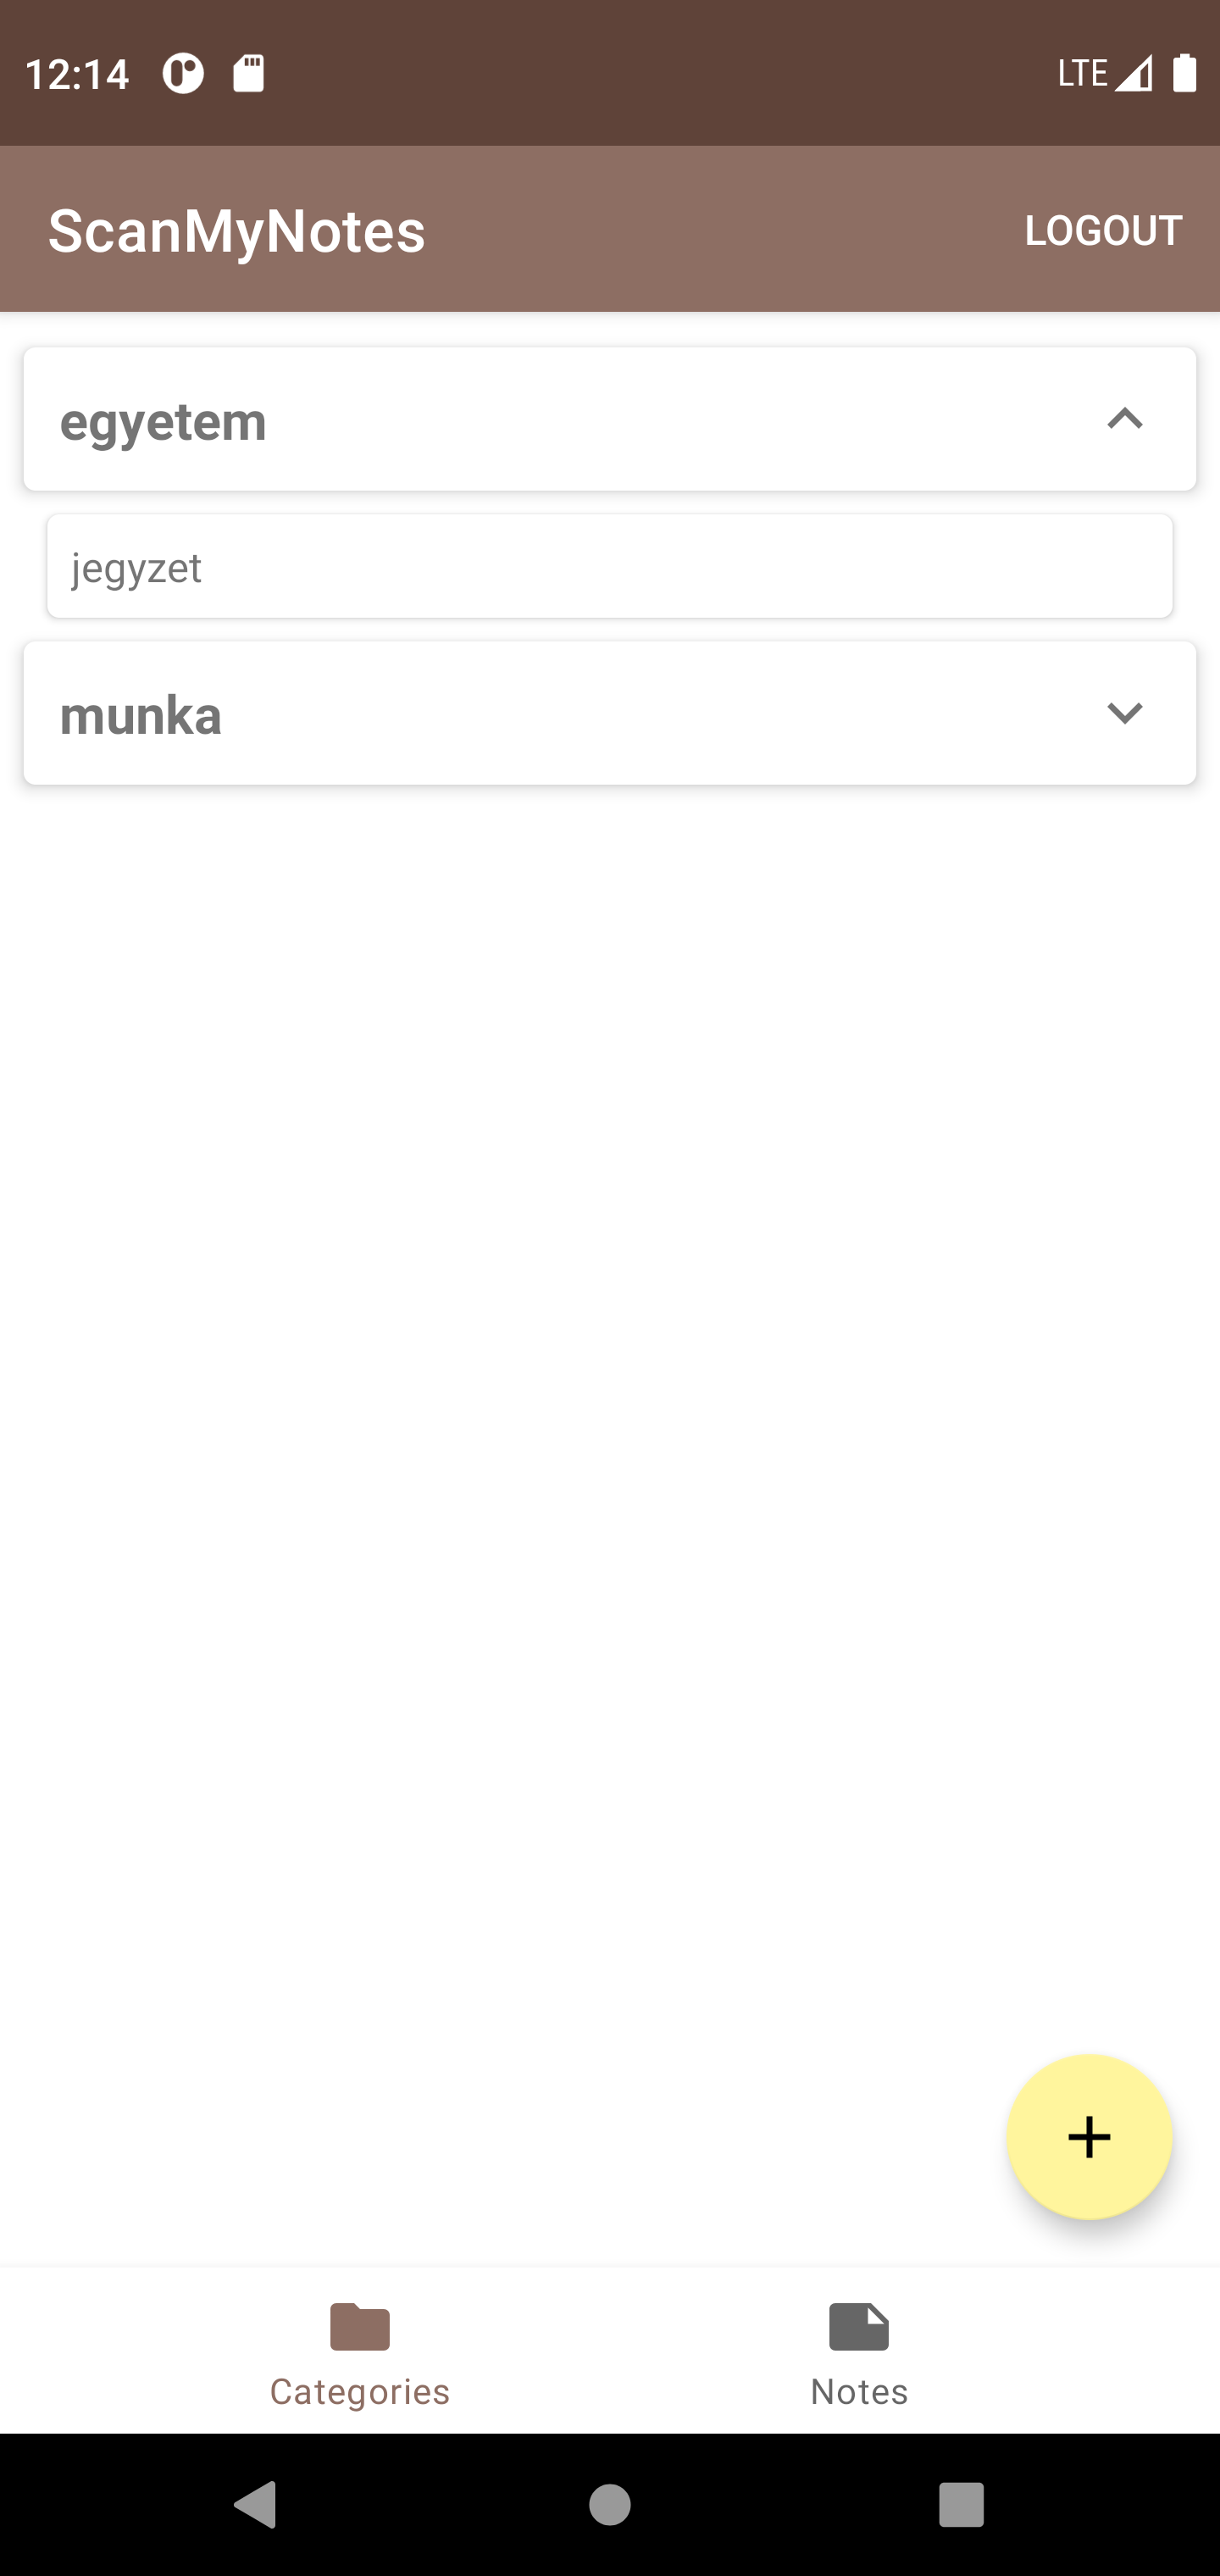
\includegraphics[width=55mm, keepaspectratio]{figures/notelist_open.png}
	\caption{Az alkalmazás kezdőlapja alapértelmezett állapotban, illetve egy kategória kibontva.}
	\label{fig:NoteListScreen}
\end{figure}

Innen számos lehetőségünk adódik navigációra az applikáción belül, kezdve a jobb felső sarokban található, meglehetősen magától értetődő kijelentkezés gombbal. Ezt megnyomva a fent leírt bejelentkezési képernyőre navigálunk, ahol adataink megadásával újra bejelentkezhetünk.

\subsection{Jegyzetlista}
A főképernyőn alul egy navigációs sávot találunk, mellyel a két különböző listamegjelenítés között tudunk váltani. Míg a \emph{Categories} opció alatt egy hierarchikusan egymás alá rendezett listát láthatunk, a \emph{Notes} opció csak a jegyzeteket tárja elénk, kategóriától függetlenül. Itt több lehetőség tárul elénk: a képernyő tetején található egy keresősáv és egy rendezés gomb. Keresni a jegyzetek címe alapján tudunk, itt gépelés közben azonnal szűkül az eredményhalmaz. A rendezés szintén a cím alapján működik, jelenleg növekvő és csökkenő betűrendet támogat az alkalmazás (\refstruc{fig:NoteListScreen2}).

\begin{figure}[!ht]
	\centering
	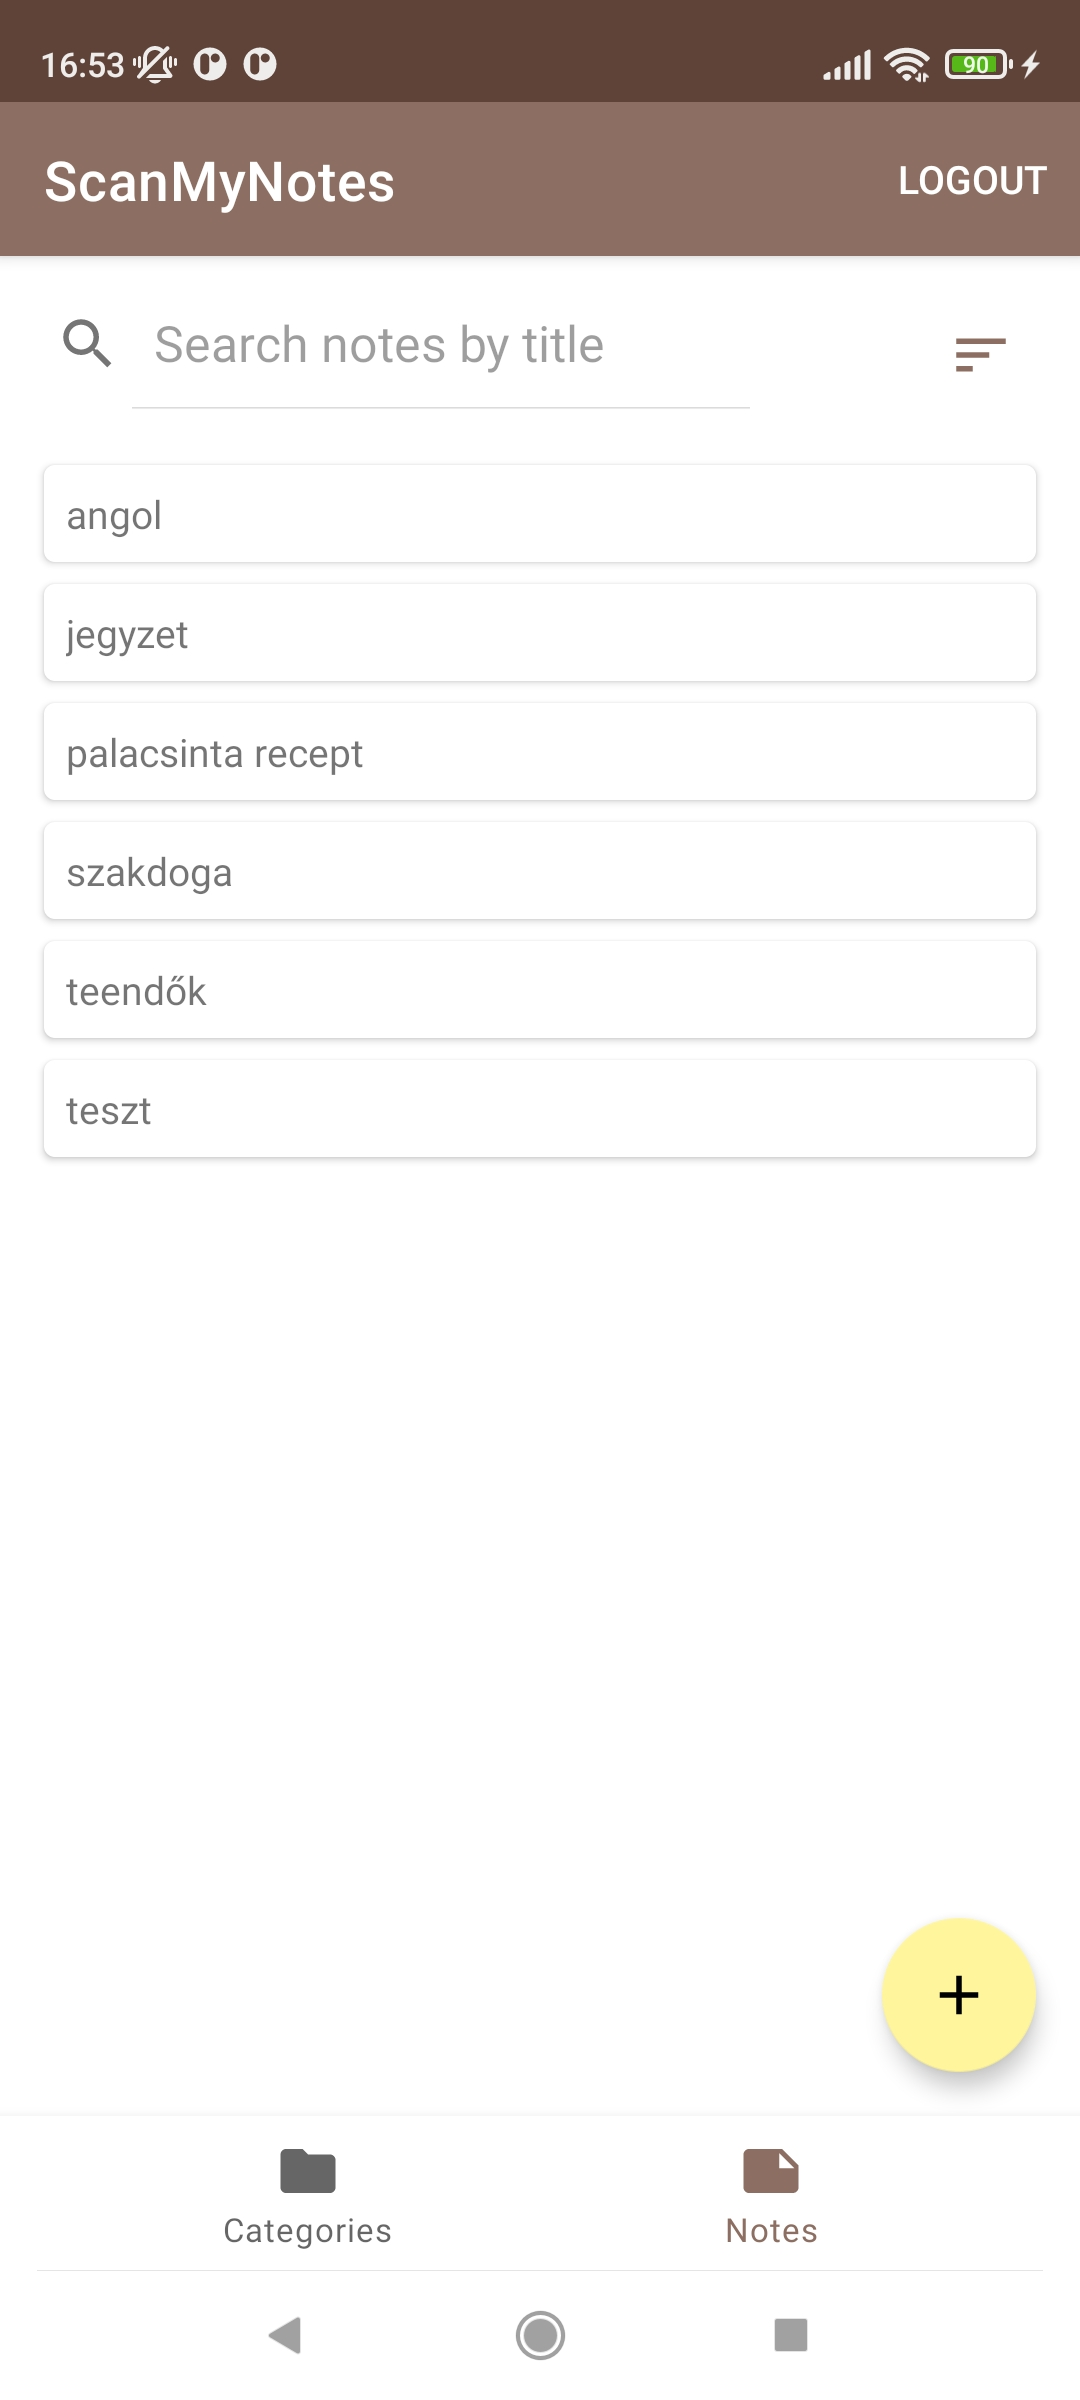
\includegraphics[width=49mm, keepaspectratio]{figures/notelist_full.jpg}
	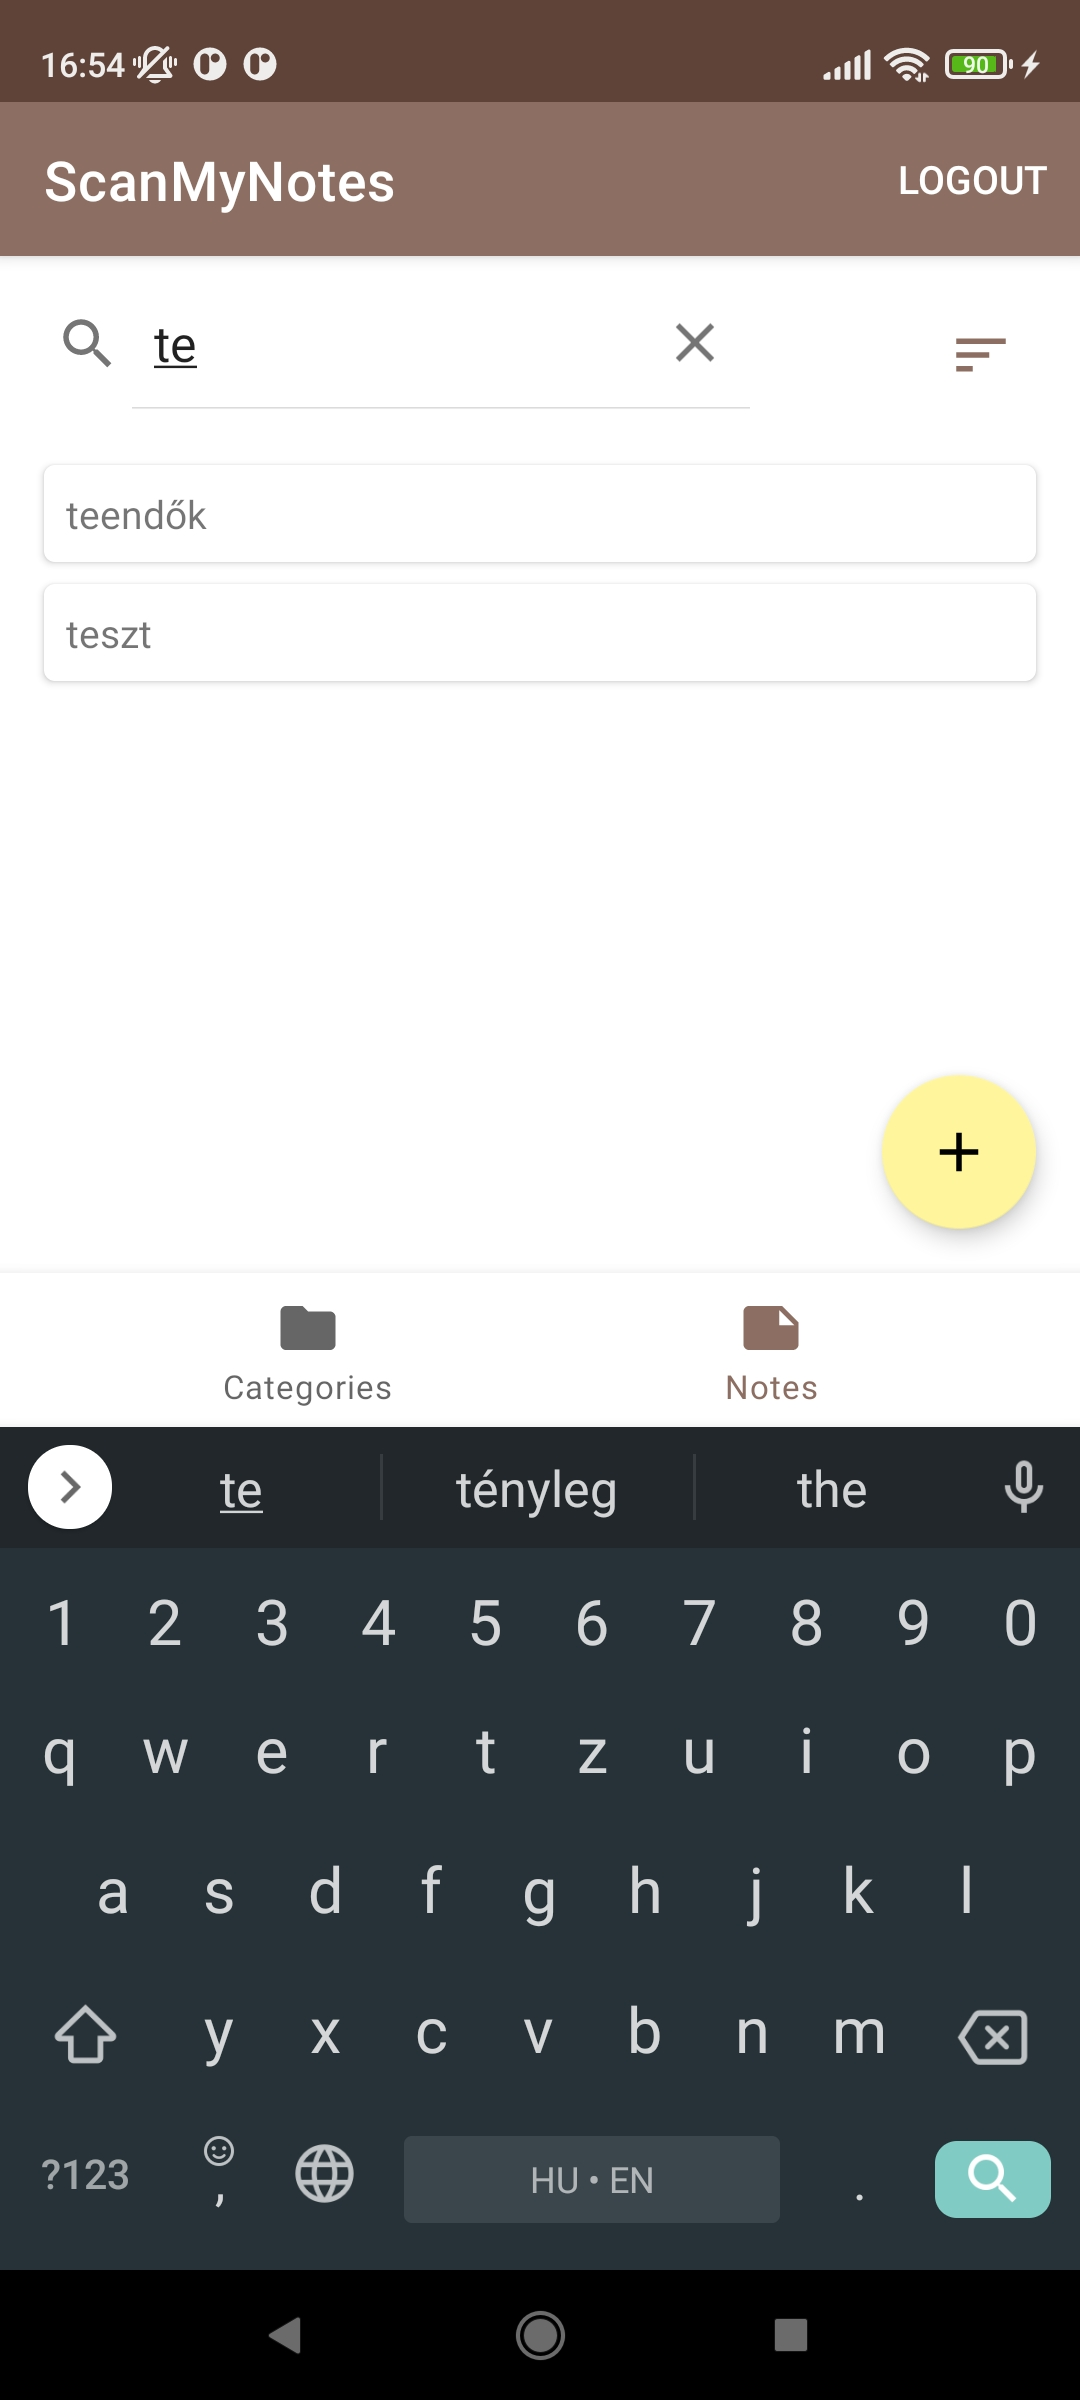
\includegraphics[width=49mm, keepaspectratio]{figures/notelist_search.jpg}
	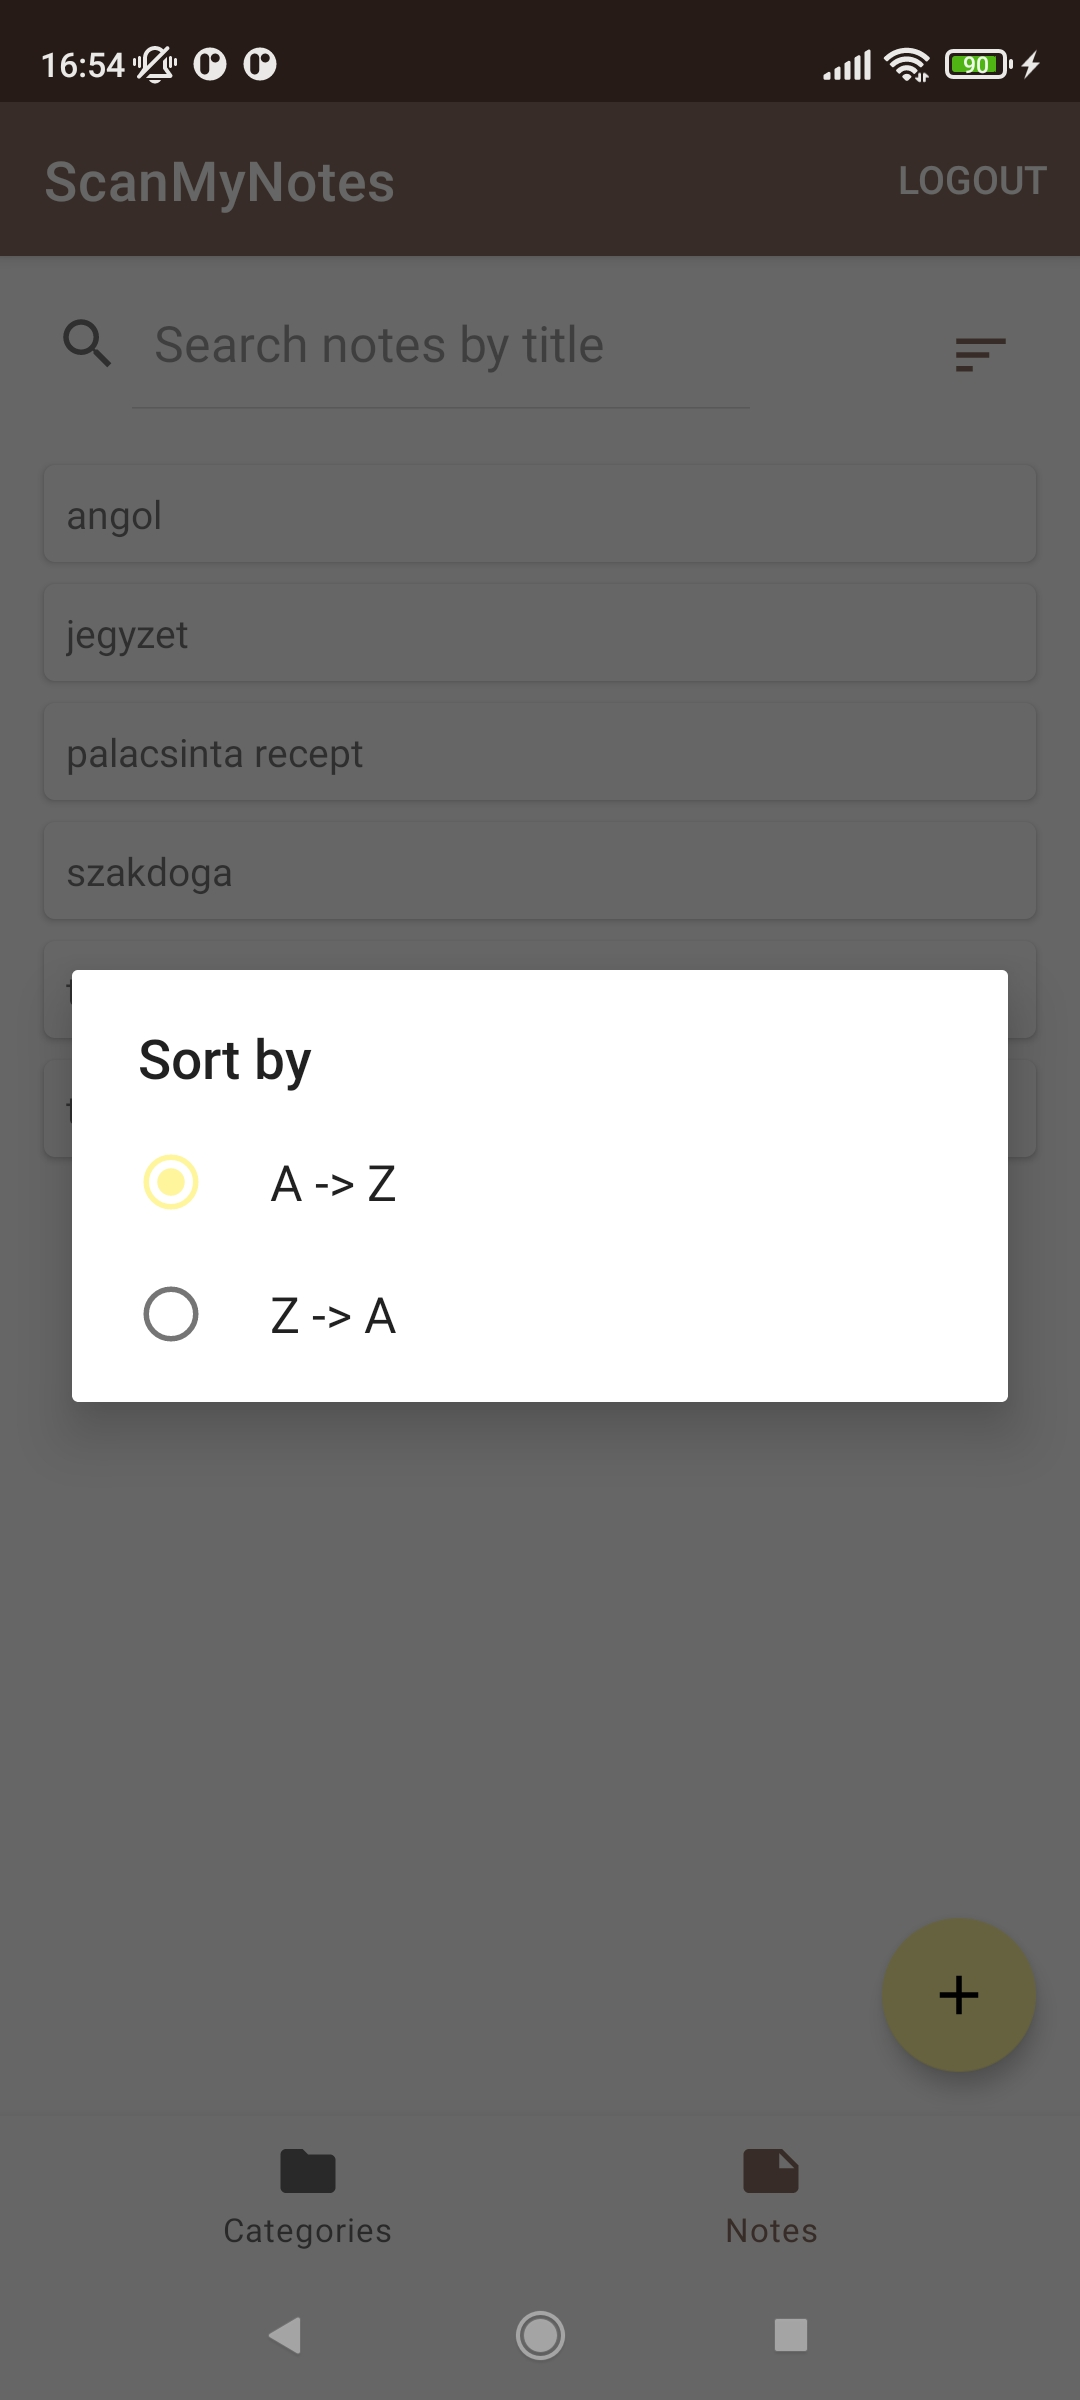
\includegraphics[width=49mm, keepaspectratio]{figures/notelist_sort.jpg}
	\caption{A jegyzetek listája, és a rajta elvégezhető műveletek.}
	\label{fig:NoteListScreen2}
\end{figure}
\newpage
\subsection{Jegyzet létrehozása}
Az alkalmazás fő funkcionalitása a jegyzetek tárolása, így elég fontos, hogy legyen lehetőség újak létrehozására. Ez a képernyő jobb alsó sarkában található plusz gombra kattintva tehető meg. Az ott megjelenő két újabb gomb közül az alsó megnyomására felugrik egy kameraablak, ahol egy fénykép készítése után megtörténik a digitalizáció, és a szerkesztési oldalra ugrunk. Itt egy cím megadásával fejezhetjük be a létrehozási folyamatot, de opcionálisan hozzárendelhetjük egy kategóriához is (\refstruc{fig:NewNoteScreen}). Amíg a cím vagy a tartalom üres, addig az alkalmazás nem fogja engedni elmenteni a jegyzetet, figyelmeztetést rak az üresen hagyott mezőre.
\begin{figure}[!ht]
	\centering
	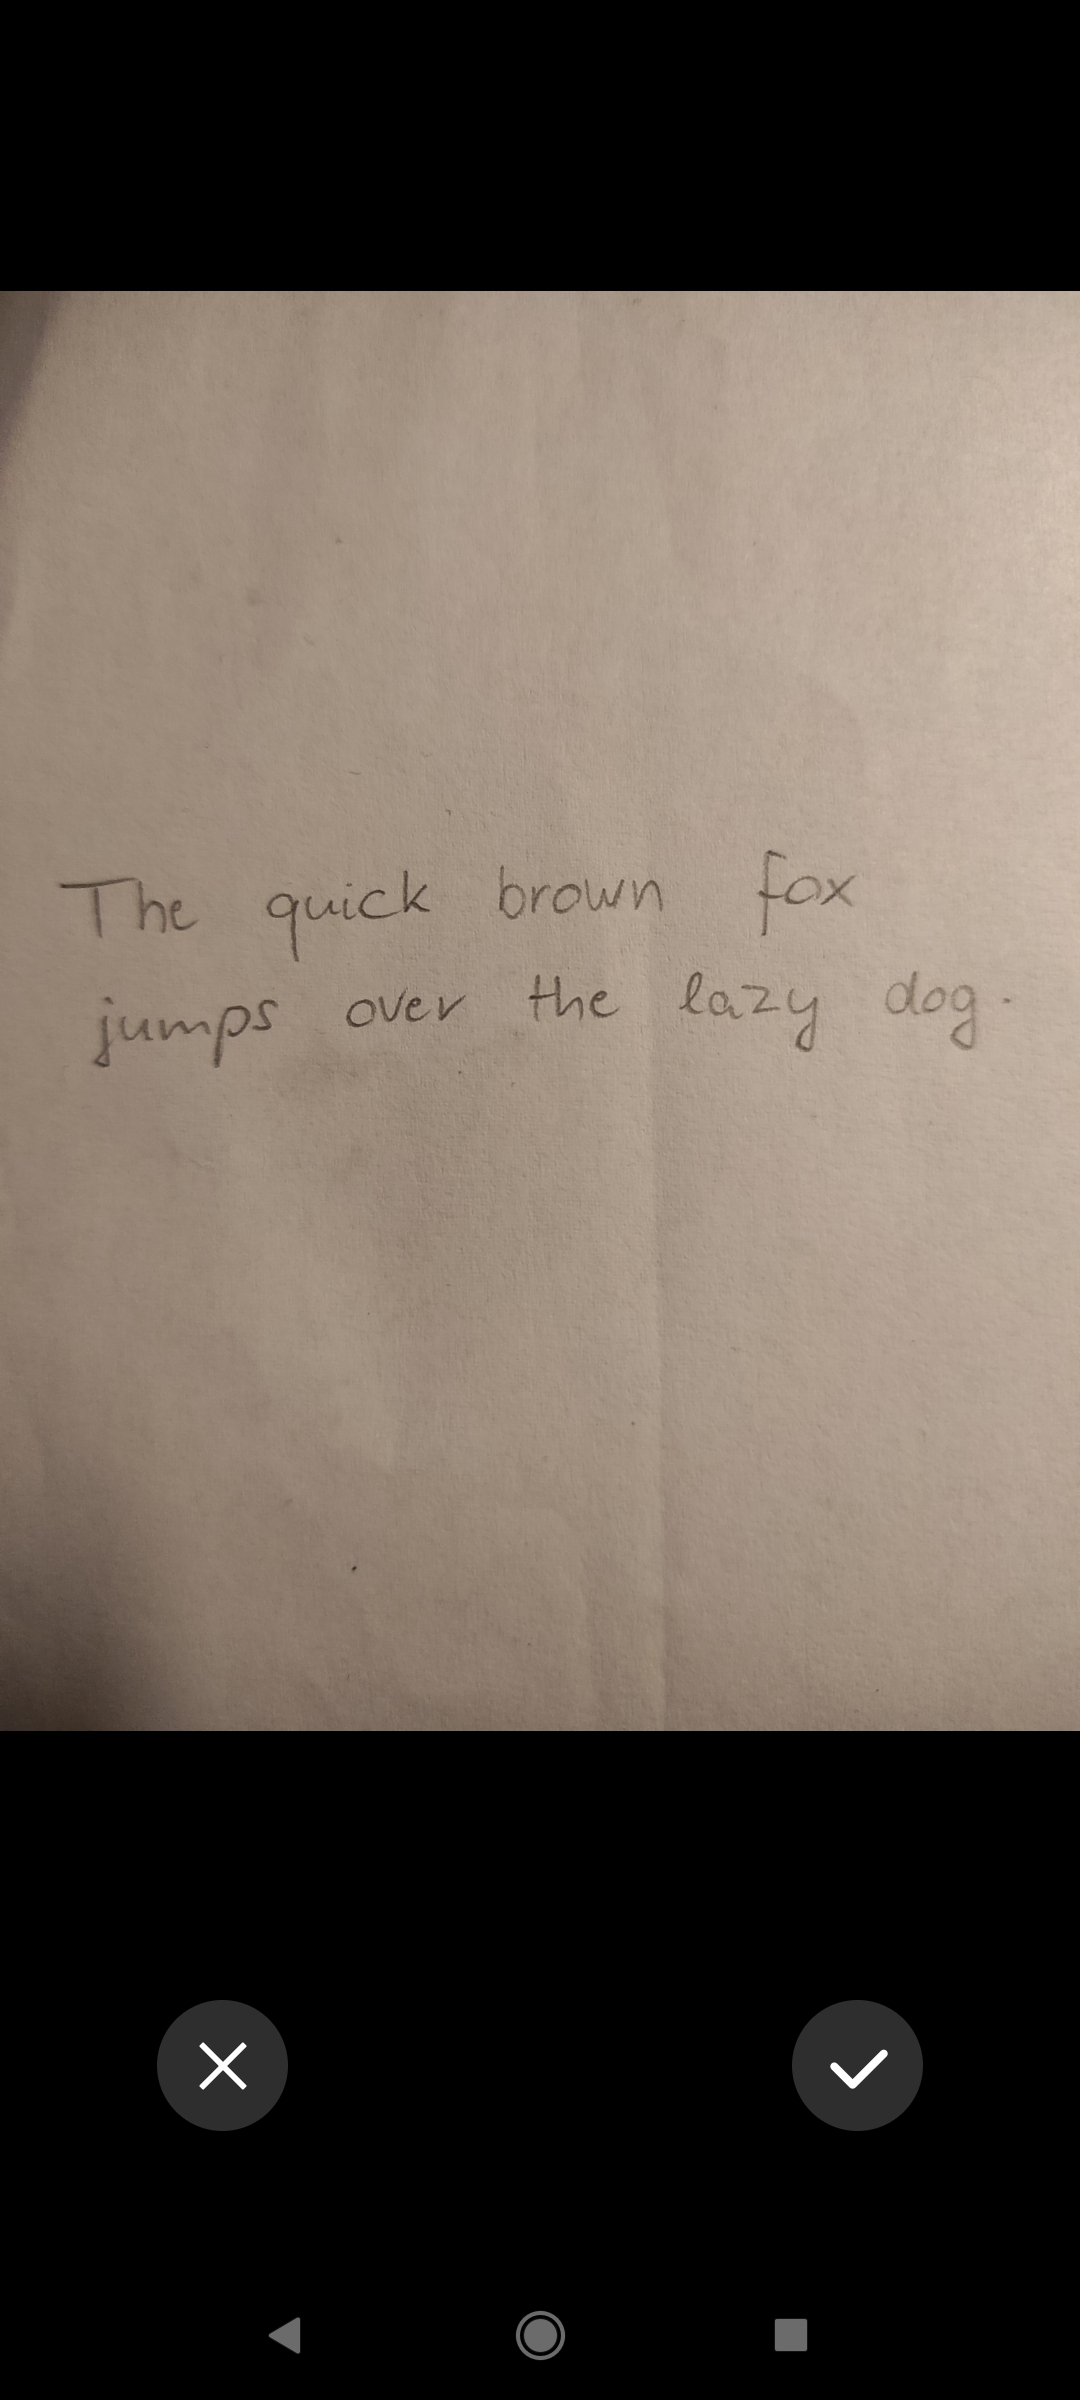
\includegraphics[width=55mm, keepaspectratio]{figures/newnote_photo.jpg}
	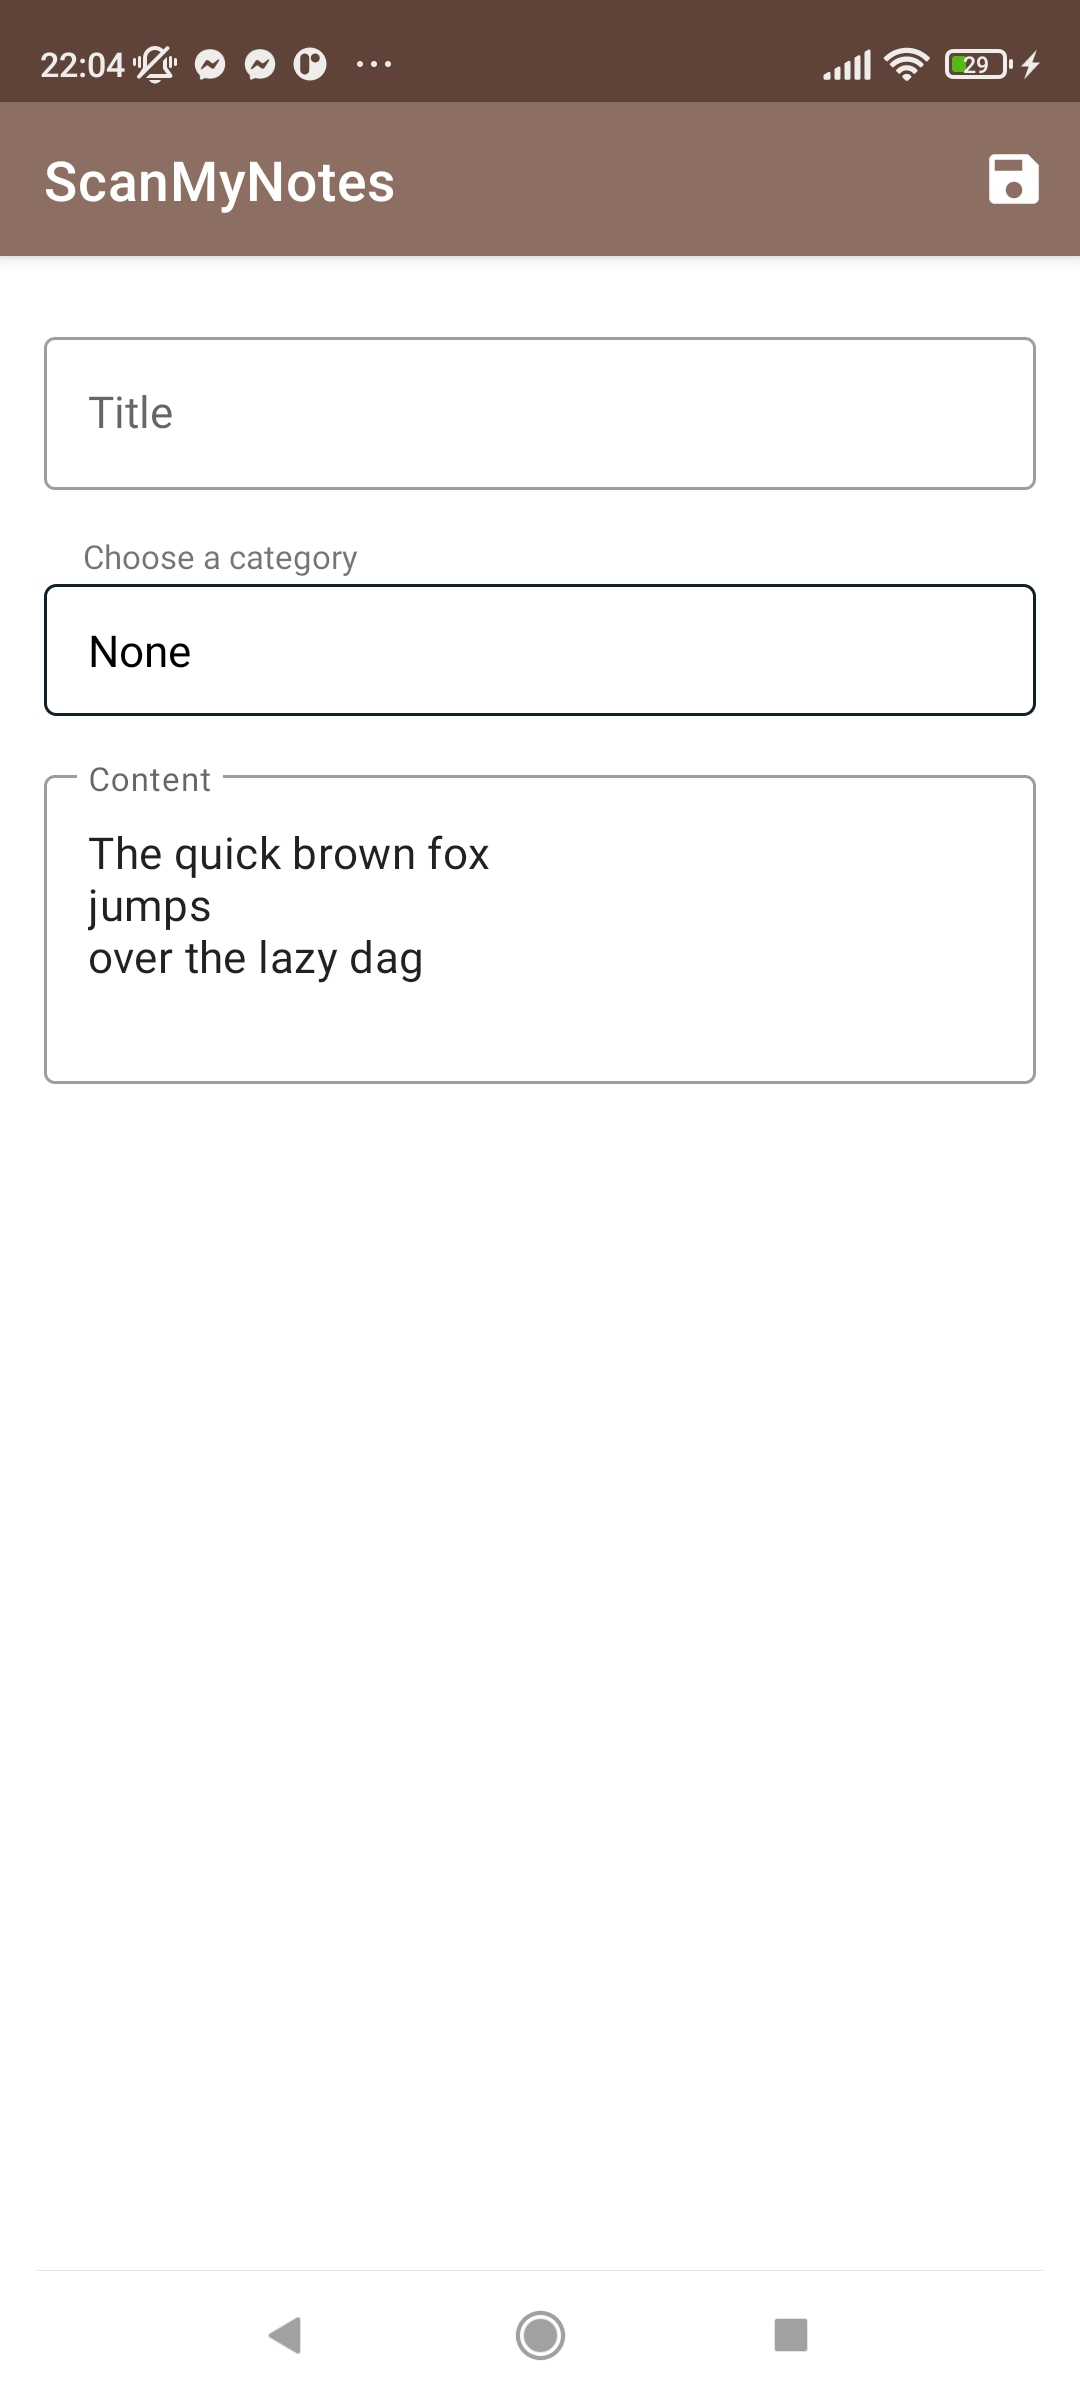
\includegraphics[width=55mm, keepaspectratio]{figures/newnote_create.jpg}
	\caption{A létrehozás során készített kép, illetve az abból kialakuló jegyzet szerkesztése.}
	\label{fig:NewNoteScreen}
\end{figure}
\newpage
\subsection{Jegyzet szerkesztése}
Amennyiben a listában egy jegyzetre kattintunk, illetve újat hozunk létre, akkor annak részletes oldalára navigálunk. Itt megtekinthetjük a tartalmát, a jobb felső sarokban található ceruza ikonra nyomva pedig szerkeszthetjük is (\refstruc{fig:NoteDetailsScreen}). Megváltoztathatjuk a címét, tartalmát, kategóriáját, a fent megjelenő pluszjel segítségével pedig készíthetünk újabb fotót, melynek szövege hozzáfűzésre kerül az eddigihez. A fentebb említett megkötések itt is érvényesek, azaz a cím és a tartalom nem lehet üres az elmentés pillanatában.

Mind megtekintési, mind szerkesztési módban elérhető a fenti sávban a szemetes ikon, mellyel törölhetjük a jegyzetet a listánkból. Vigyázat, ez a művelet nem visszafordítható!

\begin{figure}[!ht]
	\centering
	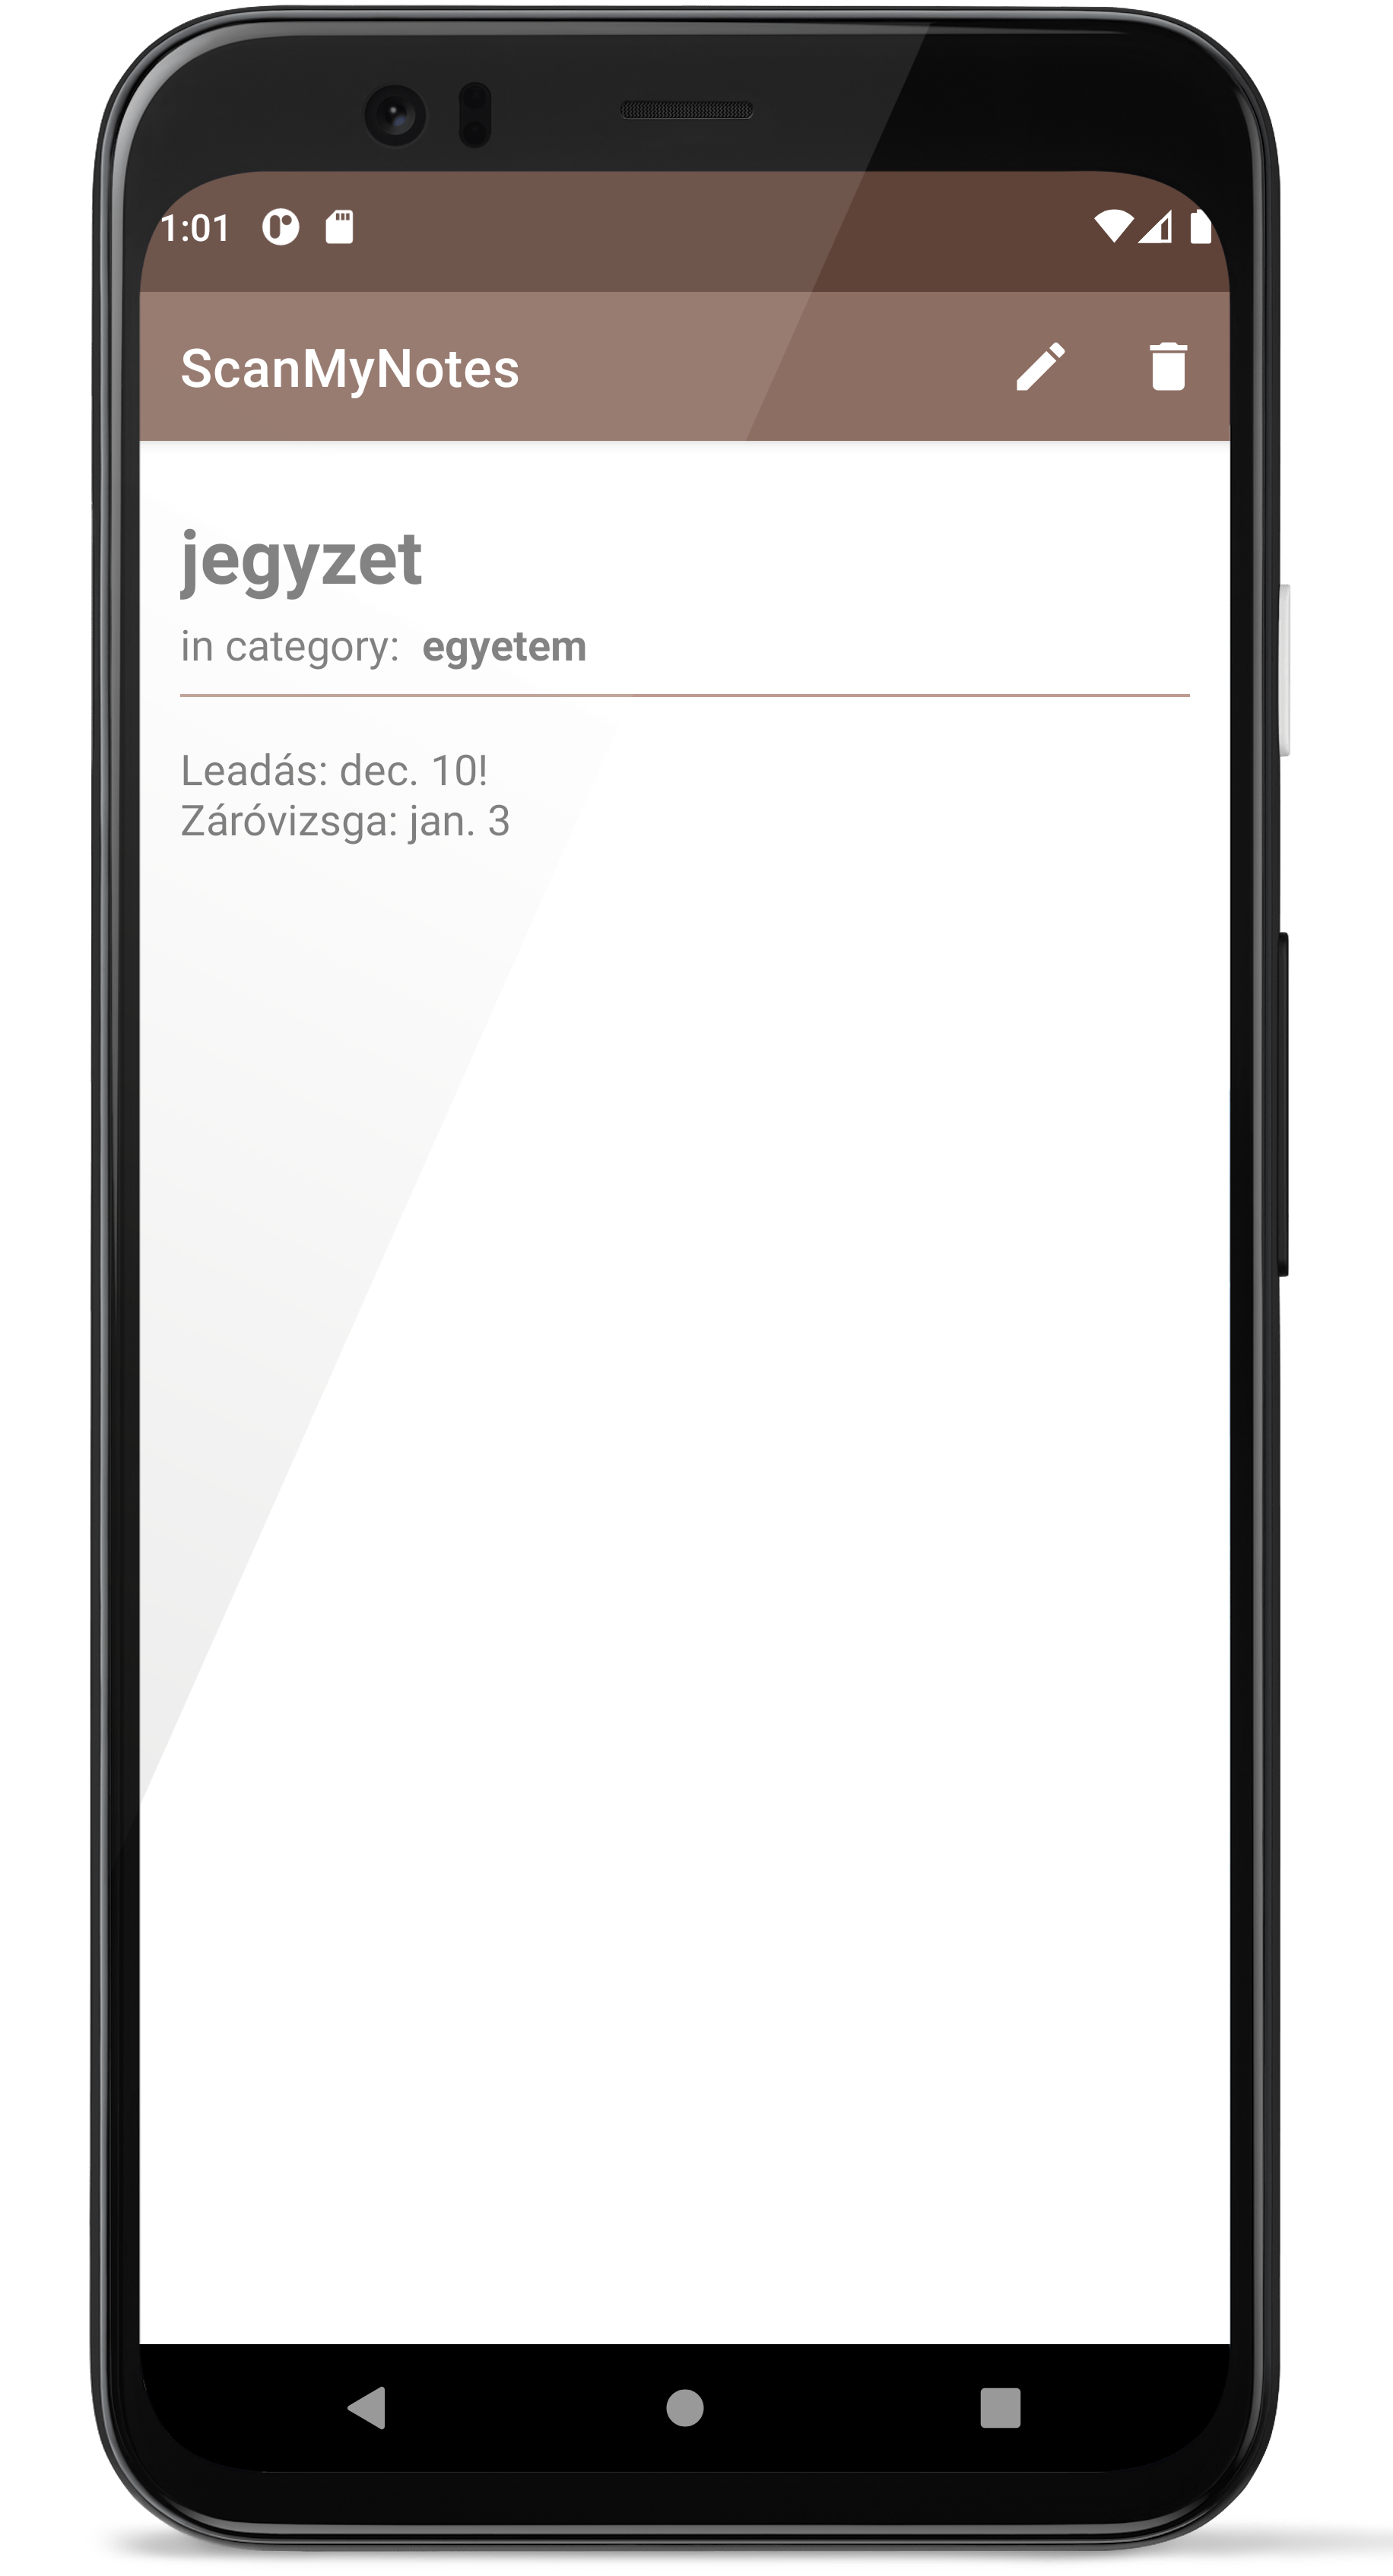
\includegraphics[width=55mm, keepaspectratio]{figures/note_view.png}
	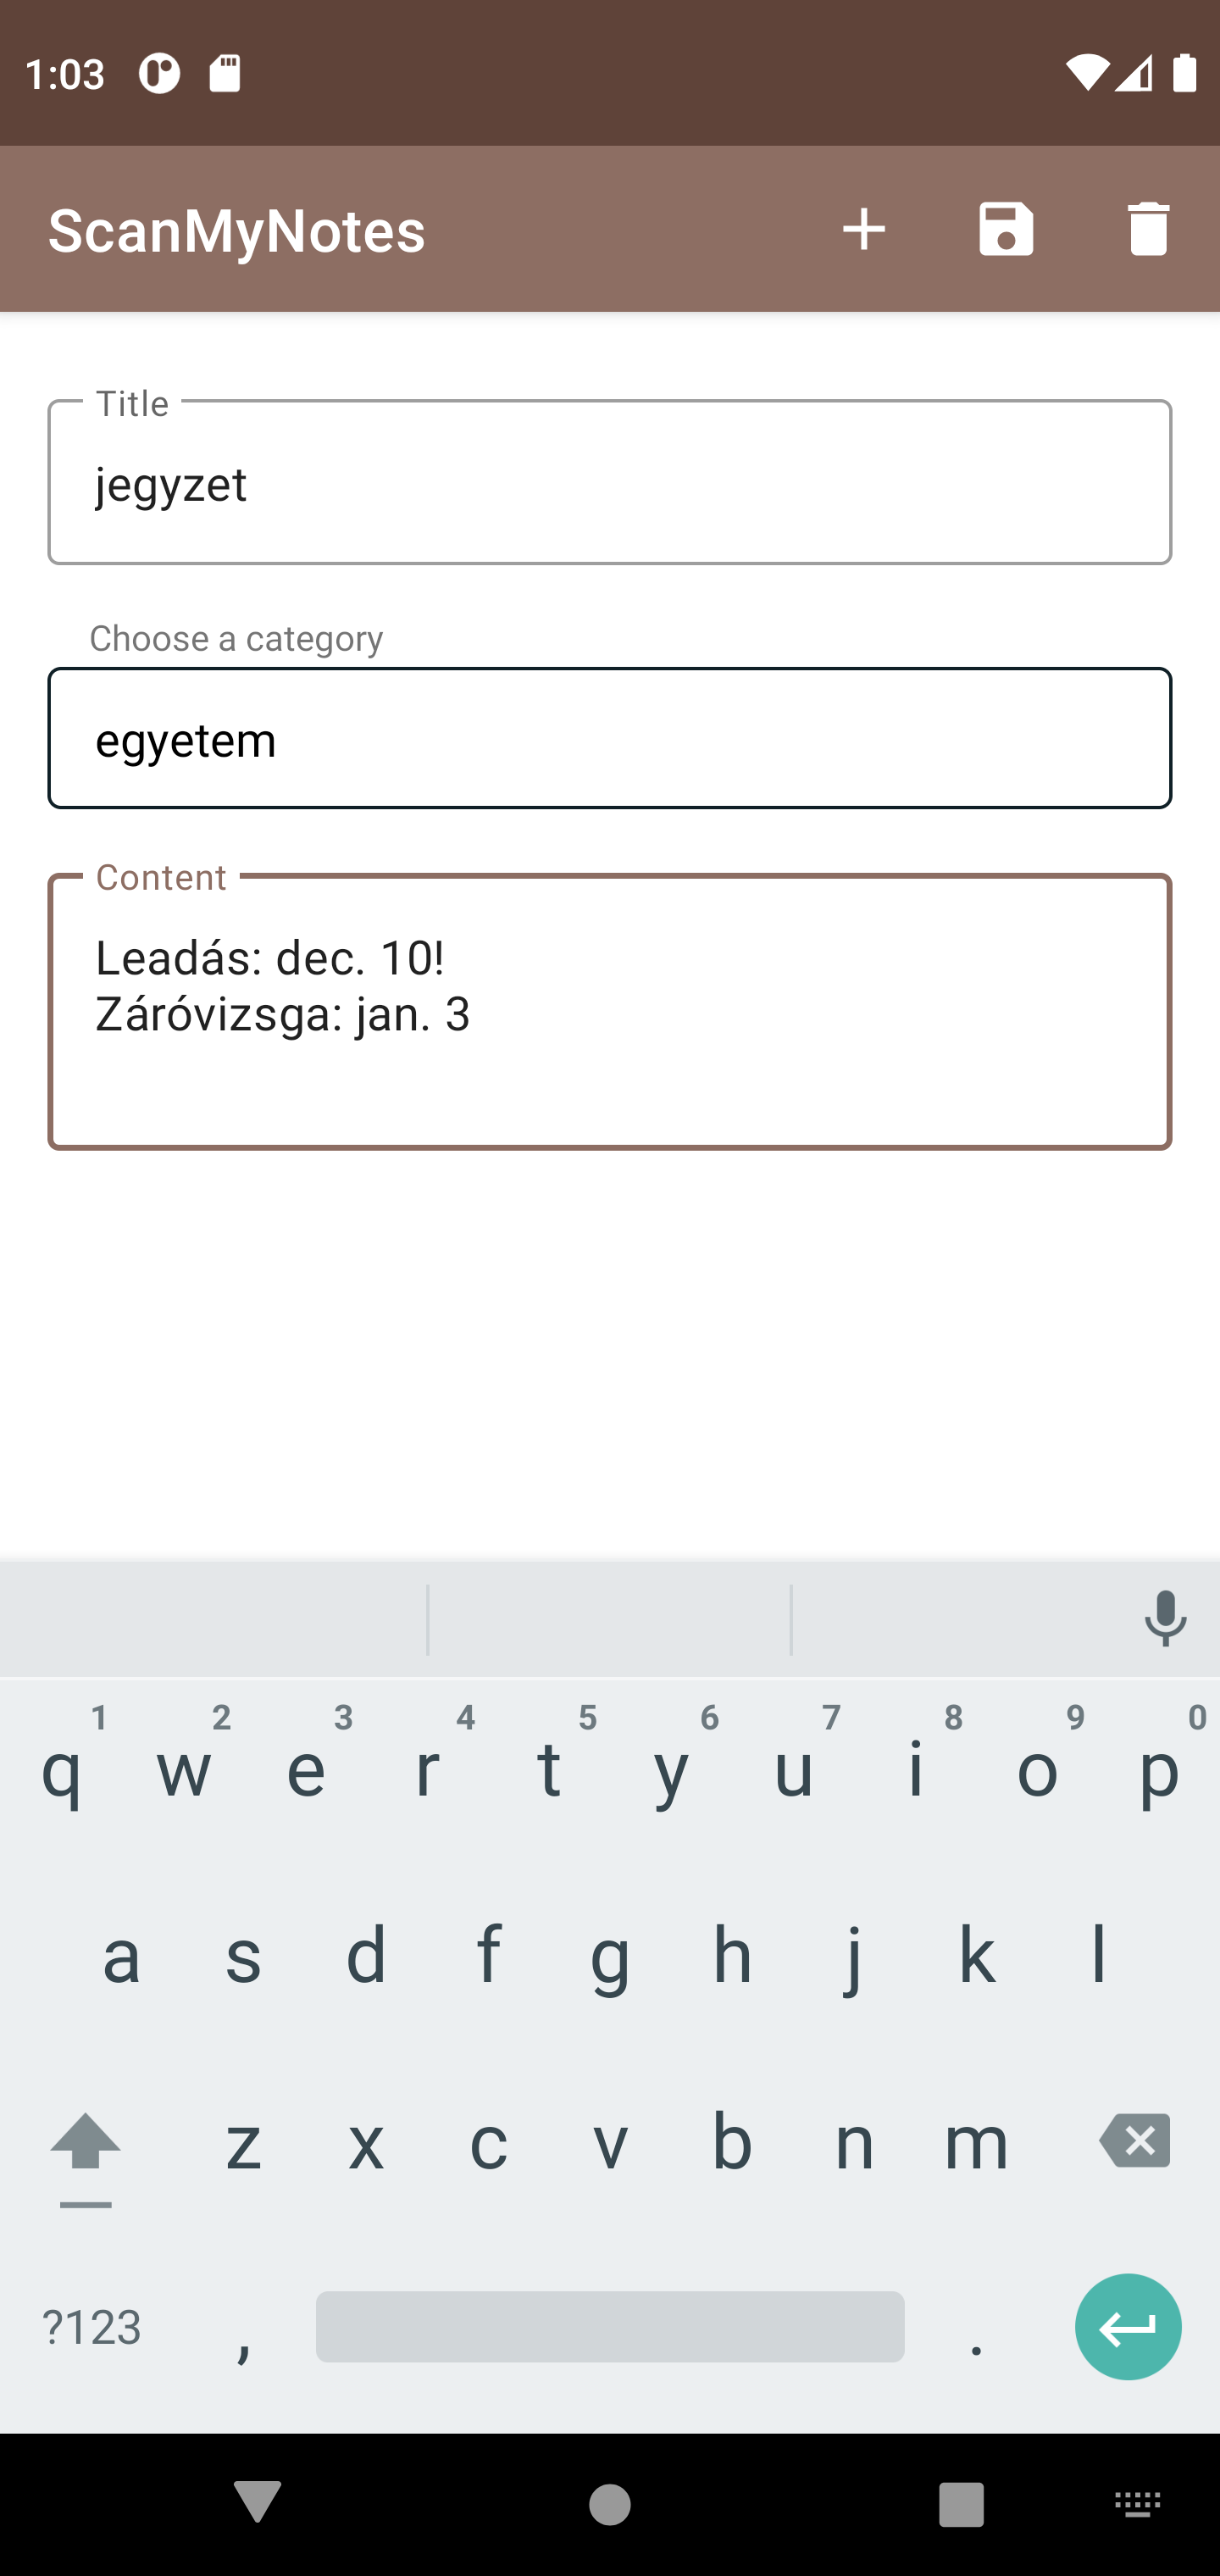
\includegraphics[width=55mm, keepaspectratio]{figures/note_edit.png}
	\caption{A jegyzet megtekintési, illetve szerkesztési képernyője.}
	\label{fig:NoteDetailsScreen}
\end{figure}
\newpage
\subsection{Kategória létrehozása}
Az alkalmazásban elérhető másik adattípus a kategória, mely rendszerezési célt szolgál. Képes magába foglalni jegyzeteket és más kategóriákat is, tetszőleges mélységben. Szintén a jobb alsó sarokban található gomb biztosítja a létrehozás lehetőségét, ám ebben az esetben a felugró két kisebb gomb közül a felsőt kell választani. Itt egy, a jegyzetkészítéshez nagyon hasonló oldalon tudunk címet és opcionálisan szülőkategóriát megadni, és amennyiben nem üres a cím mezője, el is menthetjük (\refstruc{fig:NewCategoryScreen}).

\begin{figure}[!ht]
	\centering
	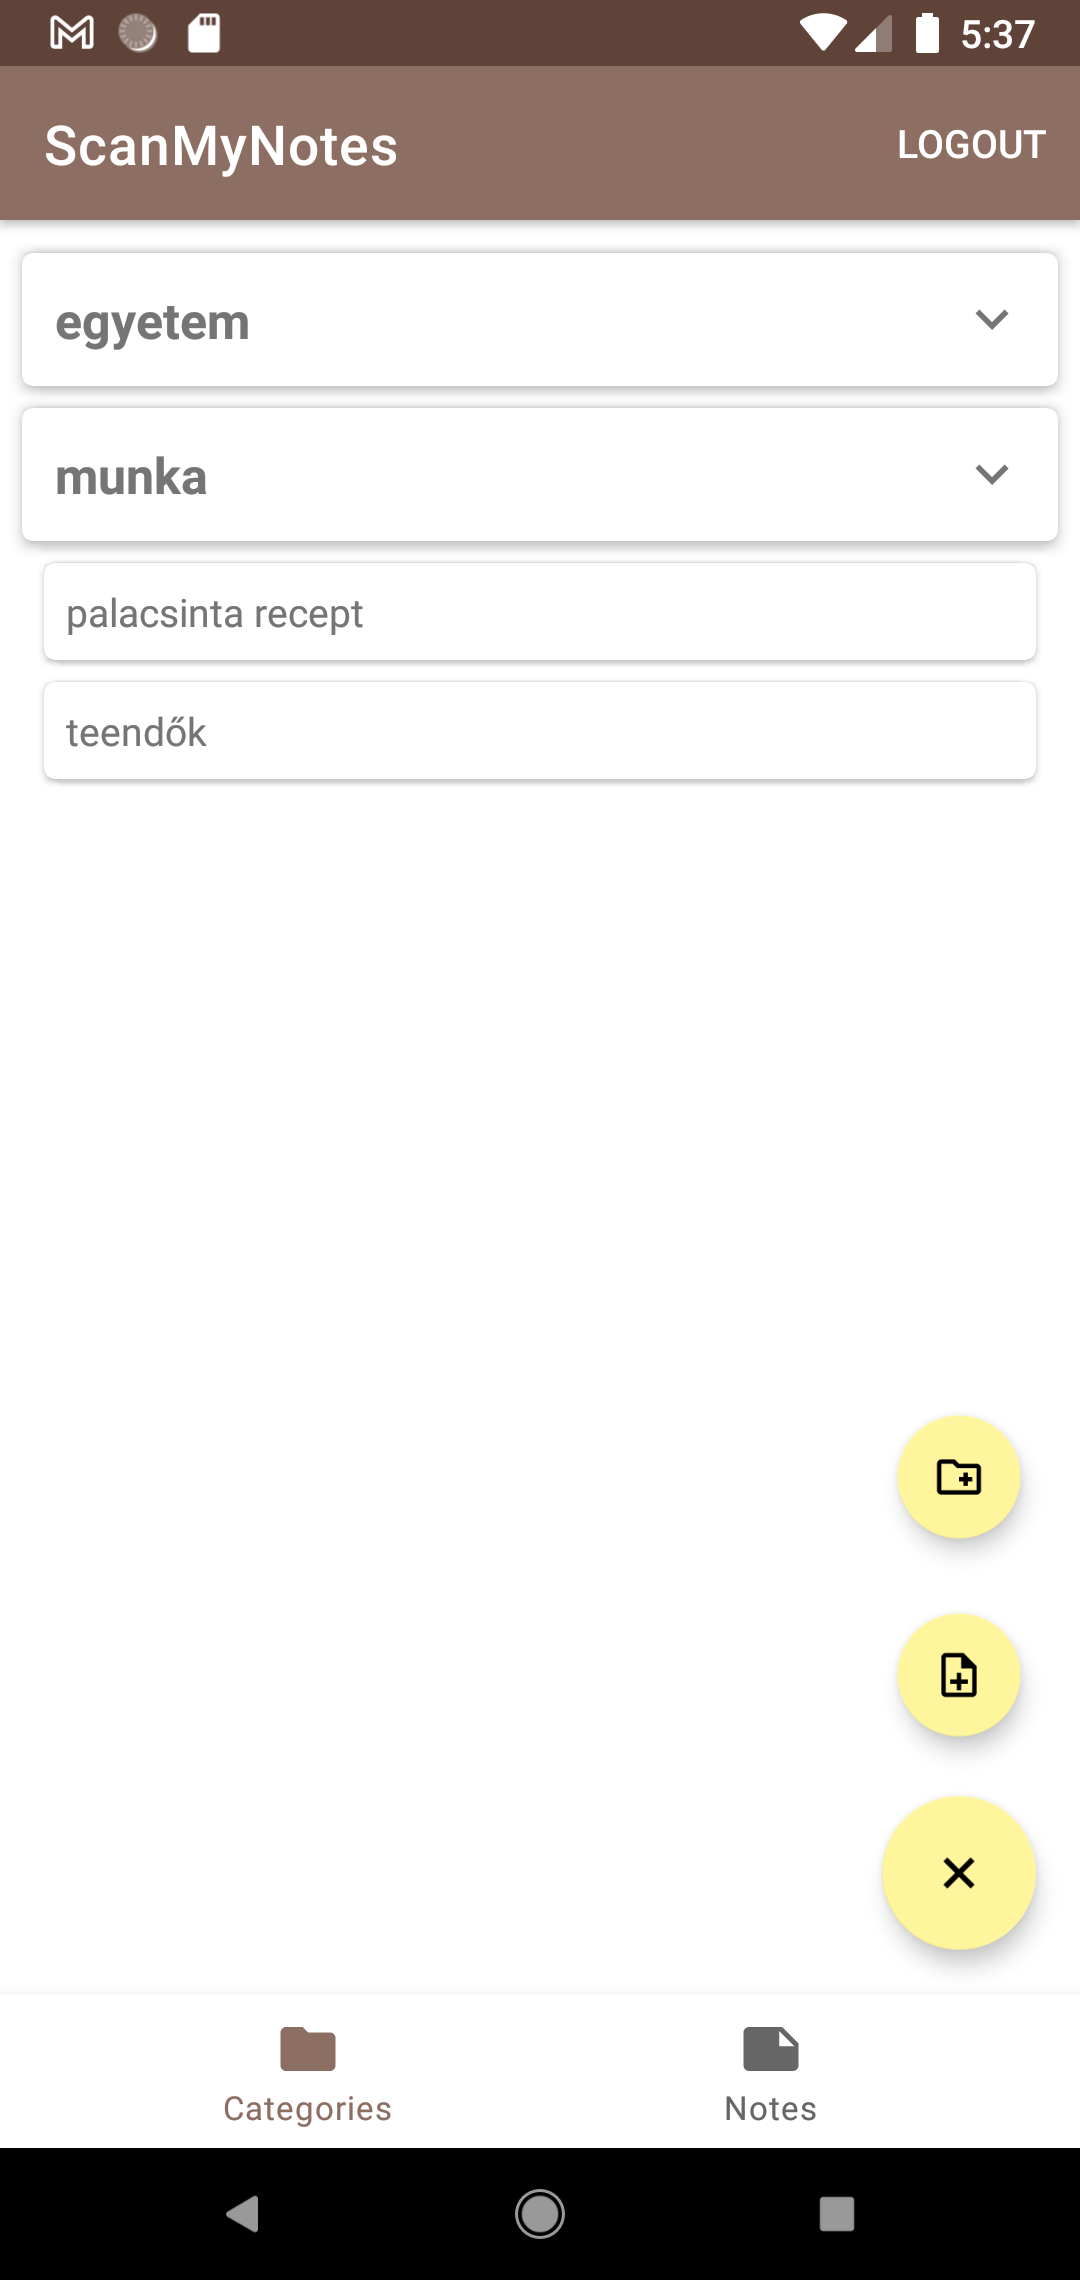
\includegraphics[width=50mm, keepaspectratio]{figures/floatingbutton_open.png}
	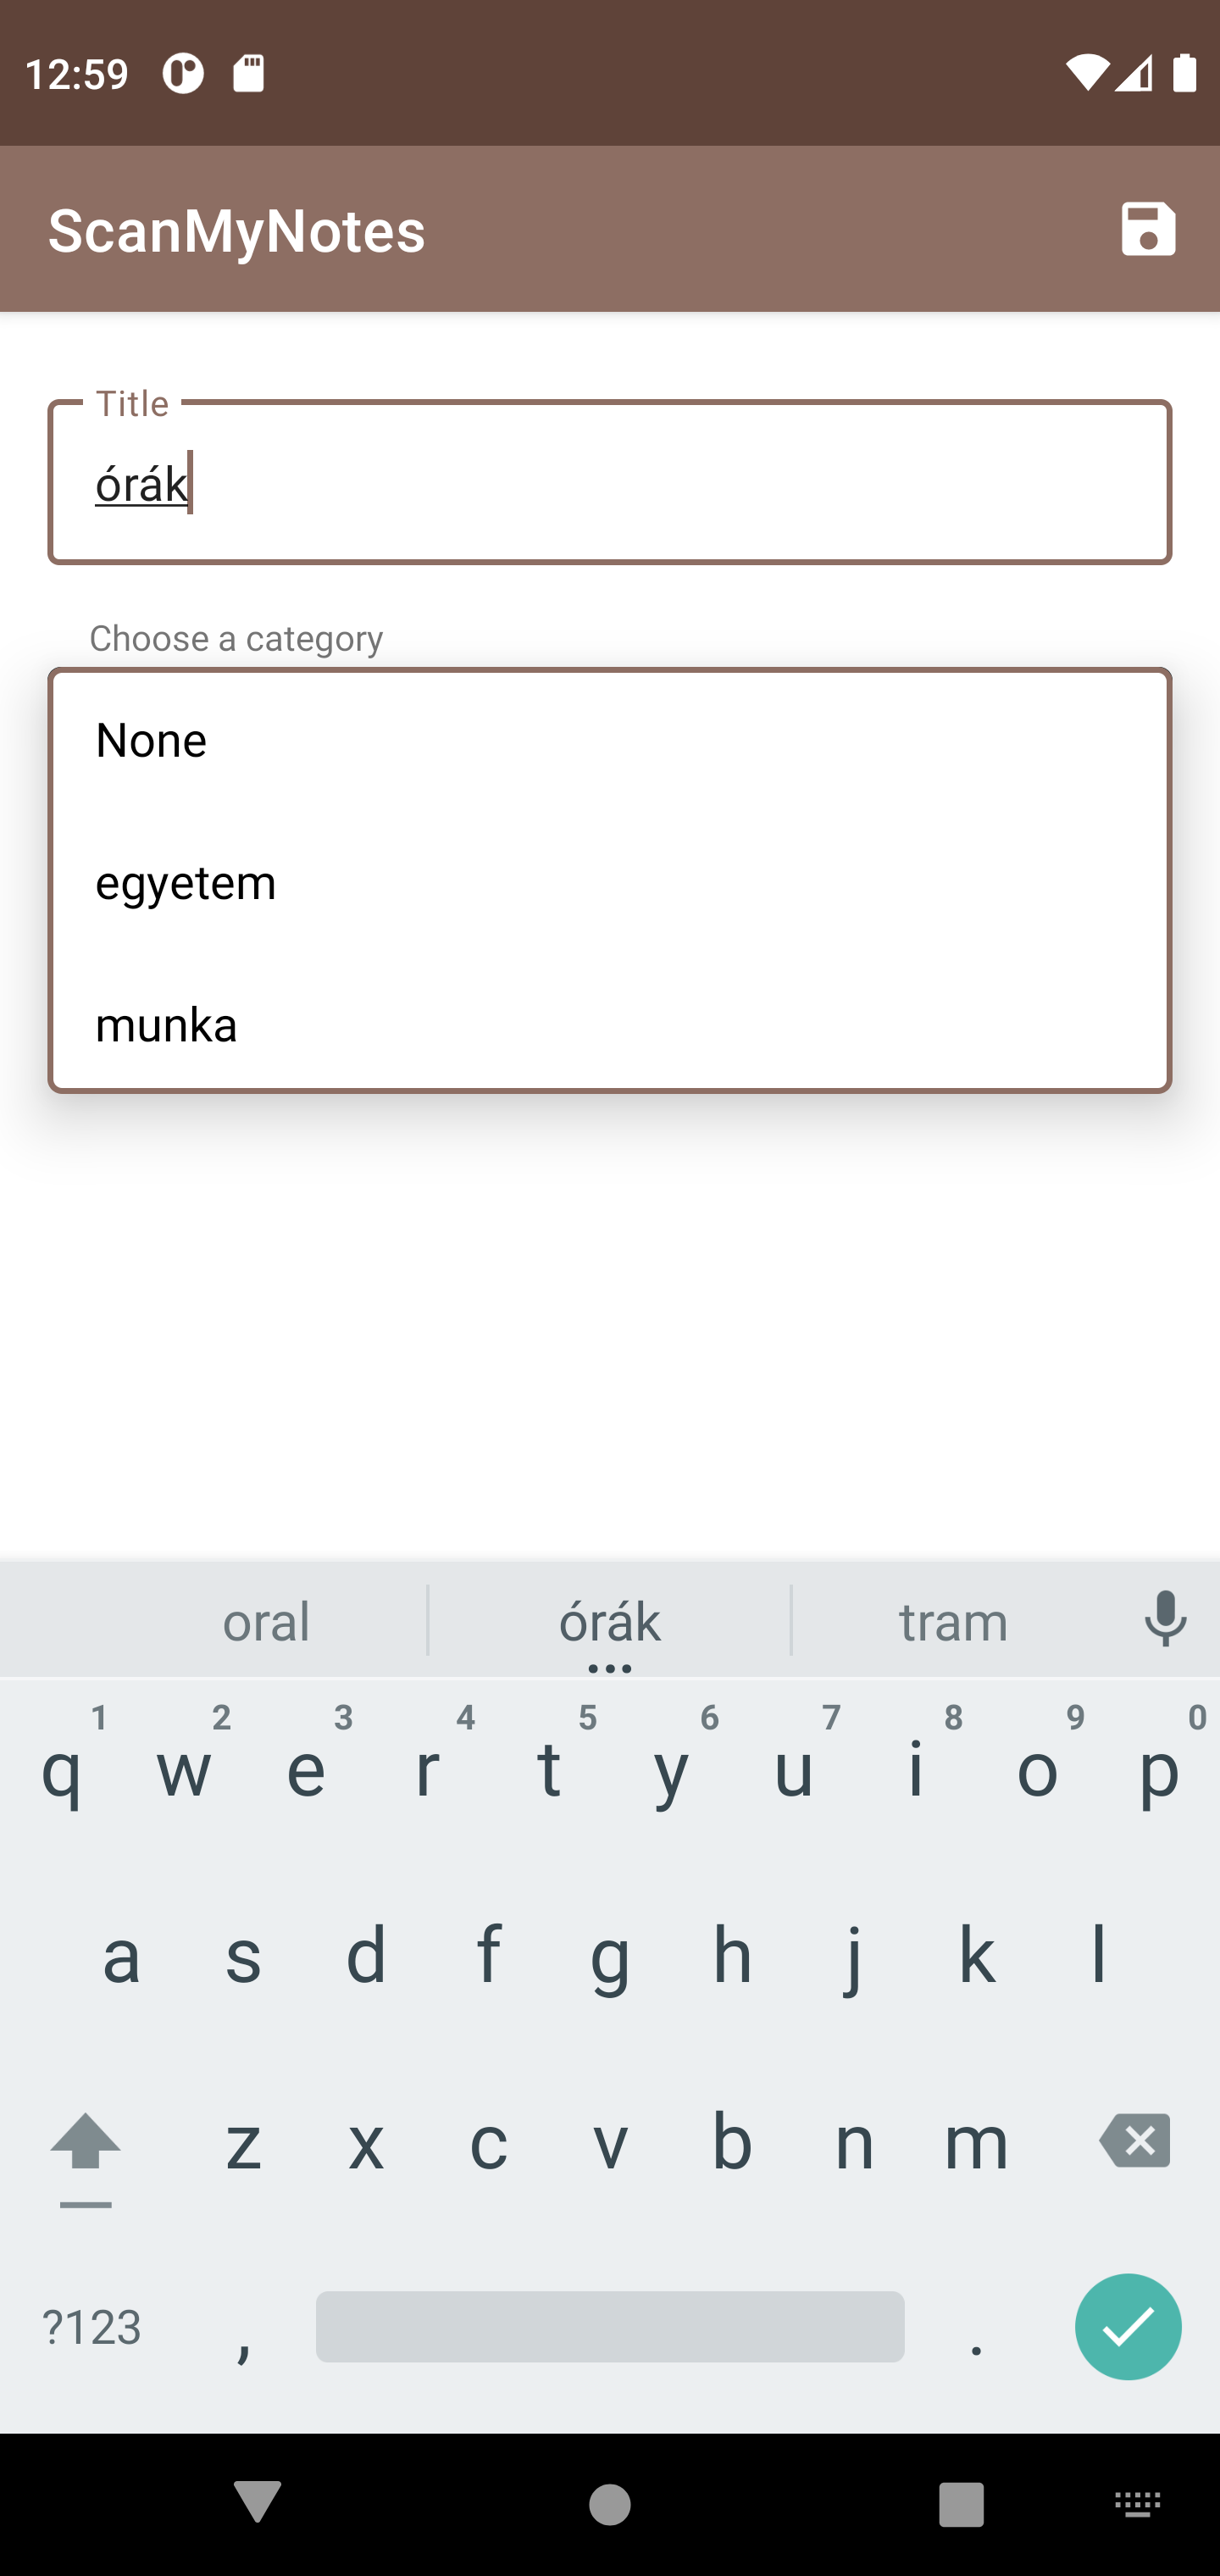
\includegraphics[width=50mm, keepaspectratio]{figures/category_save.png}
	\caption{A létrehozás gomb kinyitott állapotban, új kategória felvétele.}
	\label{fig:NewCategoryScreen}
\end{figure}
\newpage
\subsection{Kategória szerkesztése}
Új kategória létrehozása után, illetve a listában egy kategóriára nyomva annak részleteit tekinthetjük meg. Itt megjelenik a címe és esetleges szülője, és jobb fent szintén található egy ceruza ikon, mely lehetővé teszi a szerkesztést (\refstruc{fig:CategoryDetailsScreen}). Hasonlóan a jegyzethez megtekintés és szerkesztés során is törölhetjük az adott kategóriát, ilyenkor egy felugró ablak figyelmeztet rá, hogy a törlés során az összes tartalmazott objektum is törlődni fog.

\begin{figure}[!ht]
	\centering
	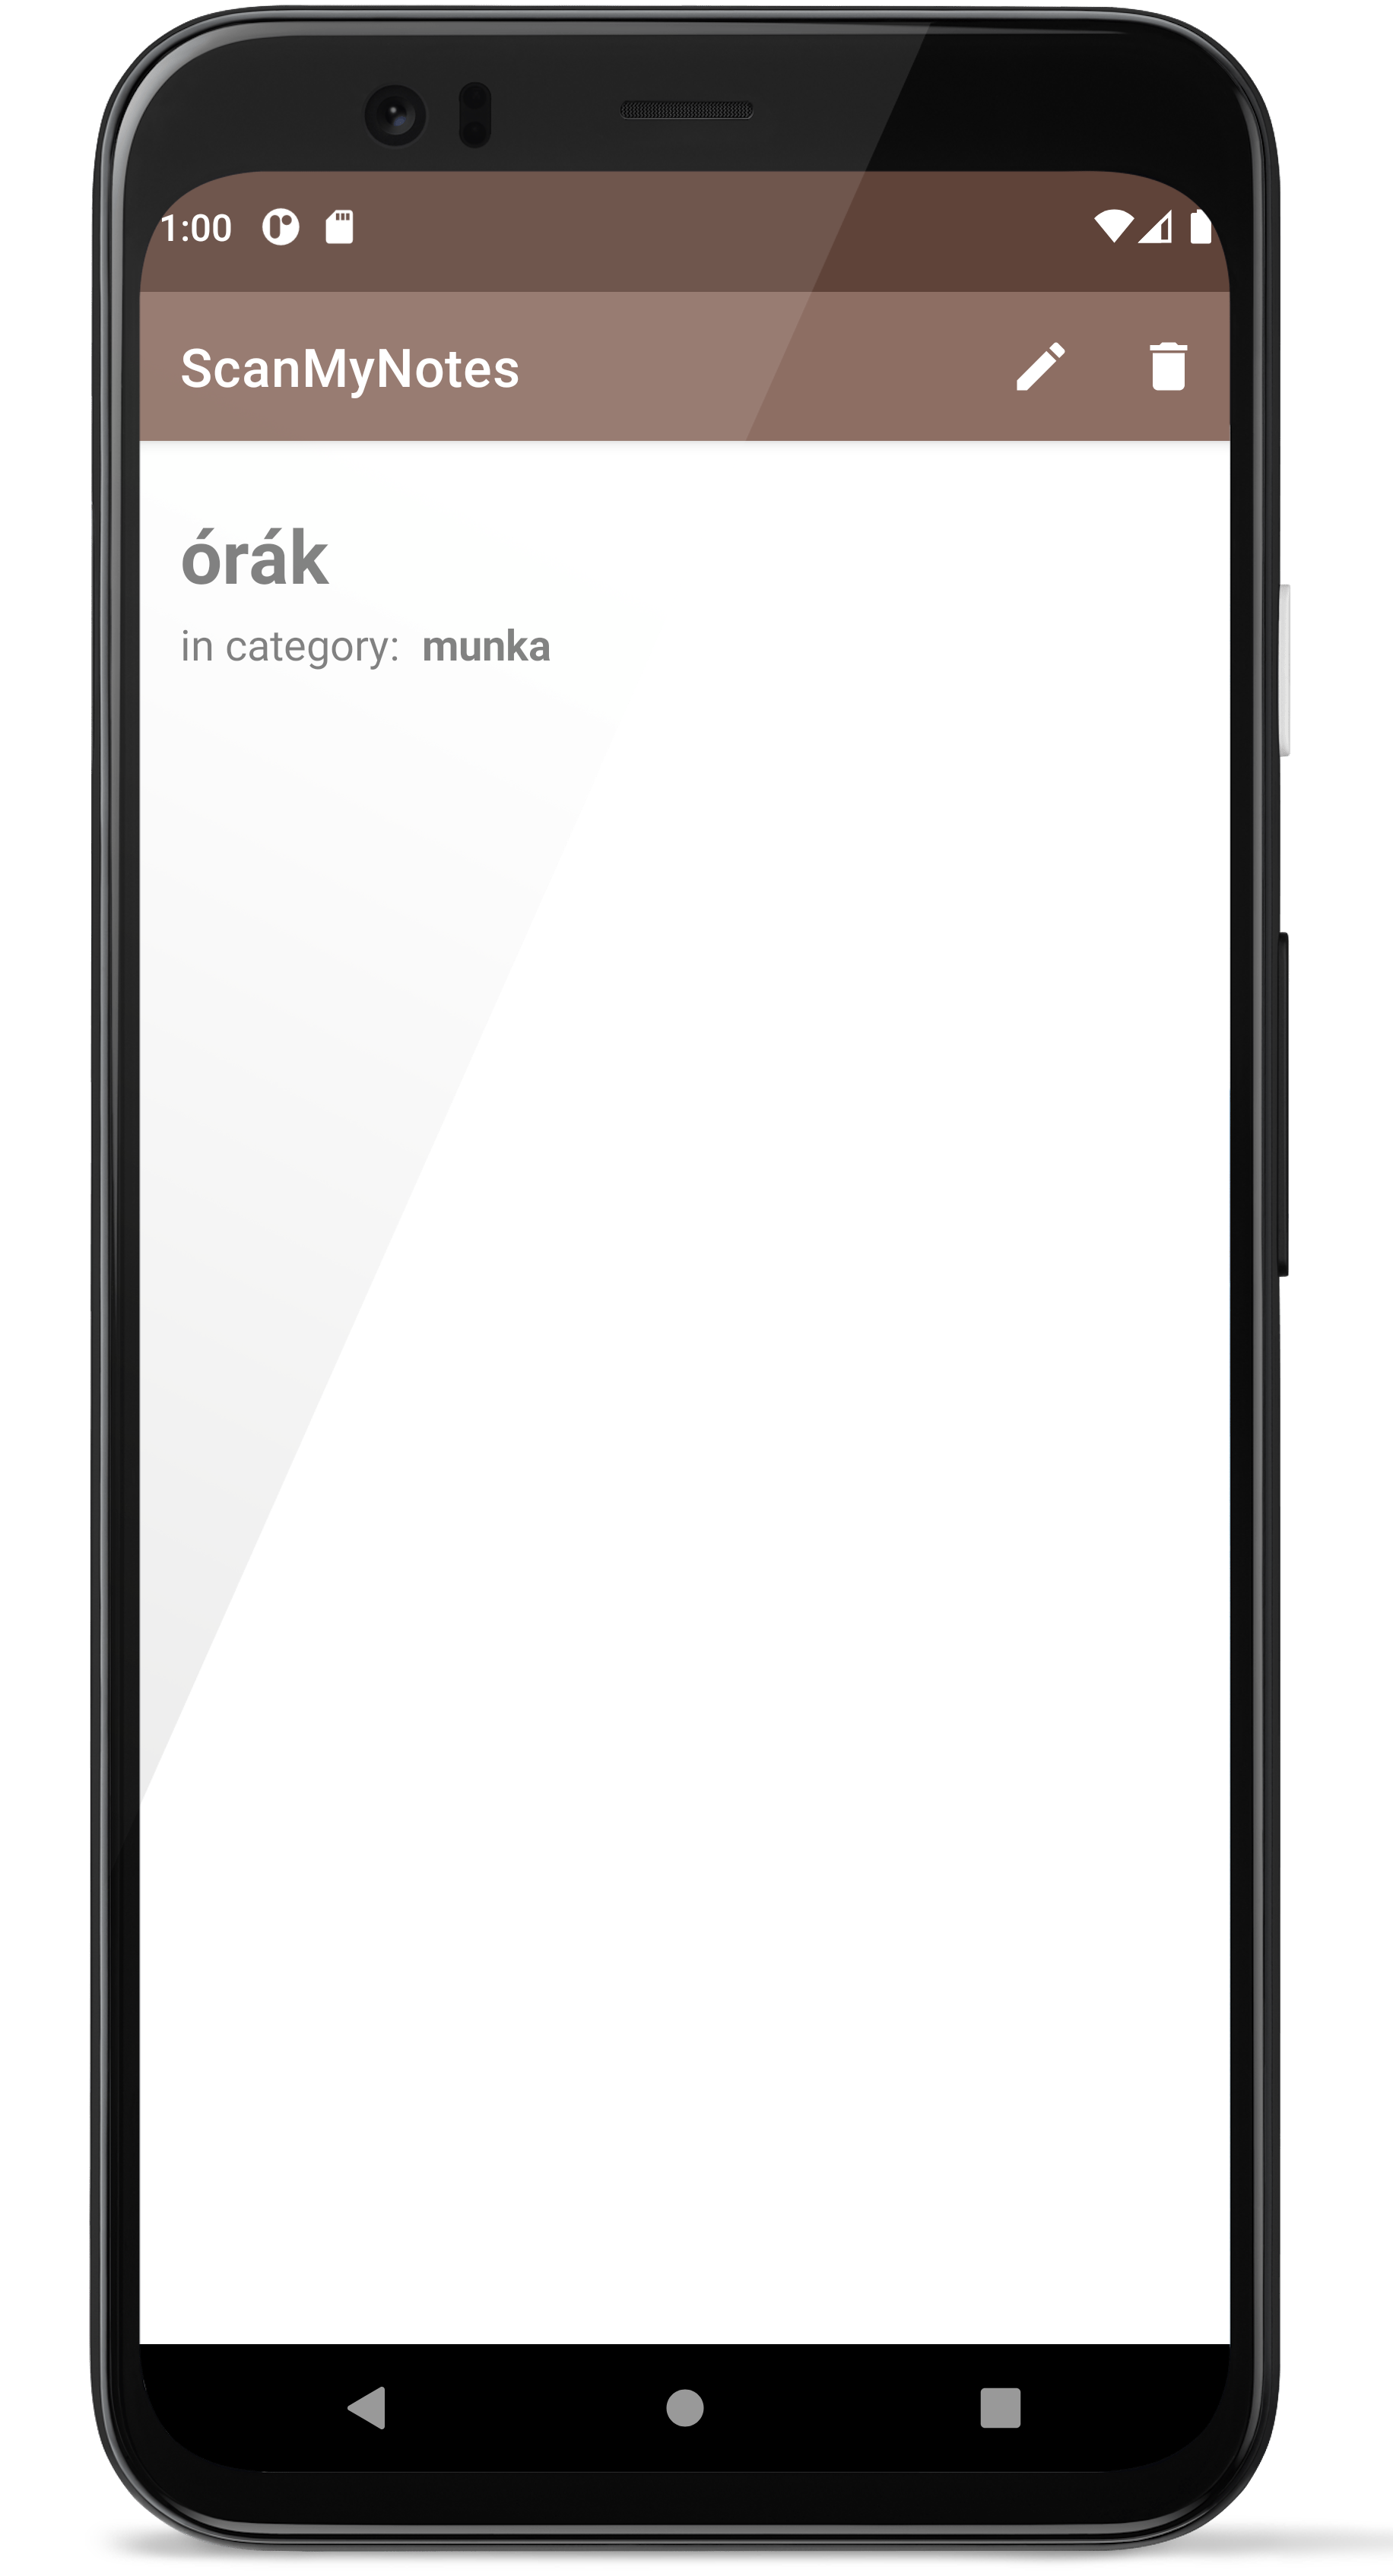
\includegraphics[width=50mm, keepaspectratio]{figures/category_view.png}
	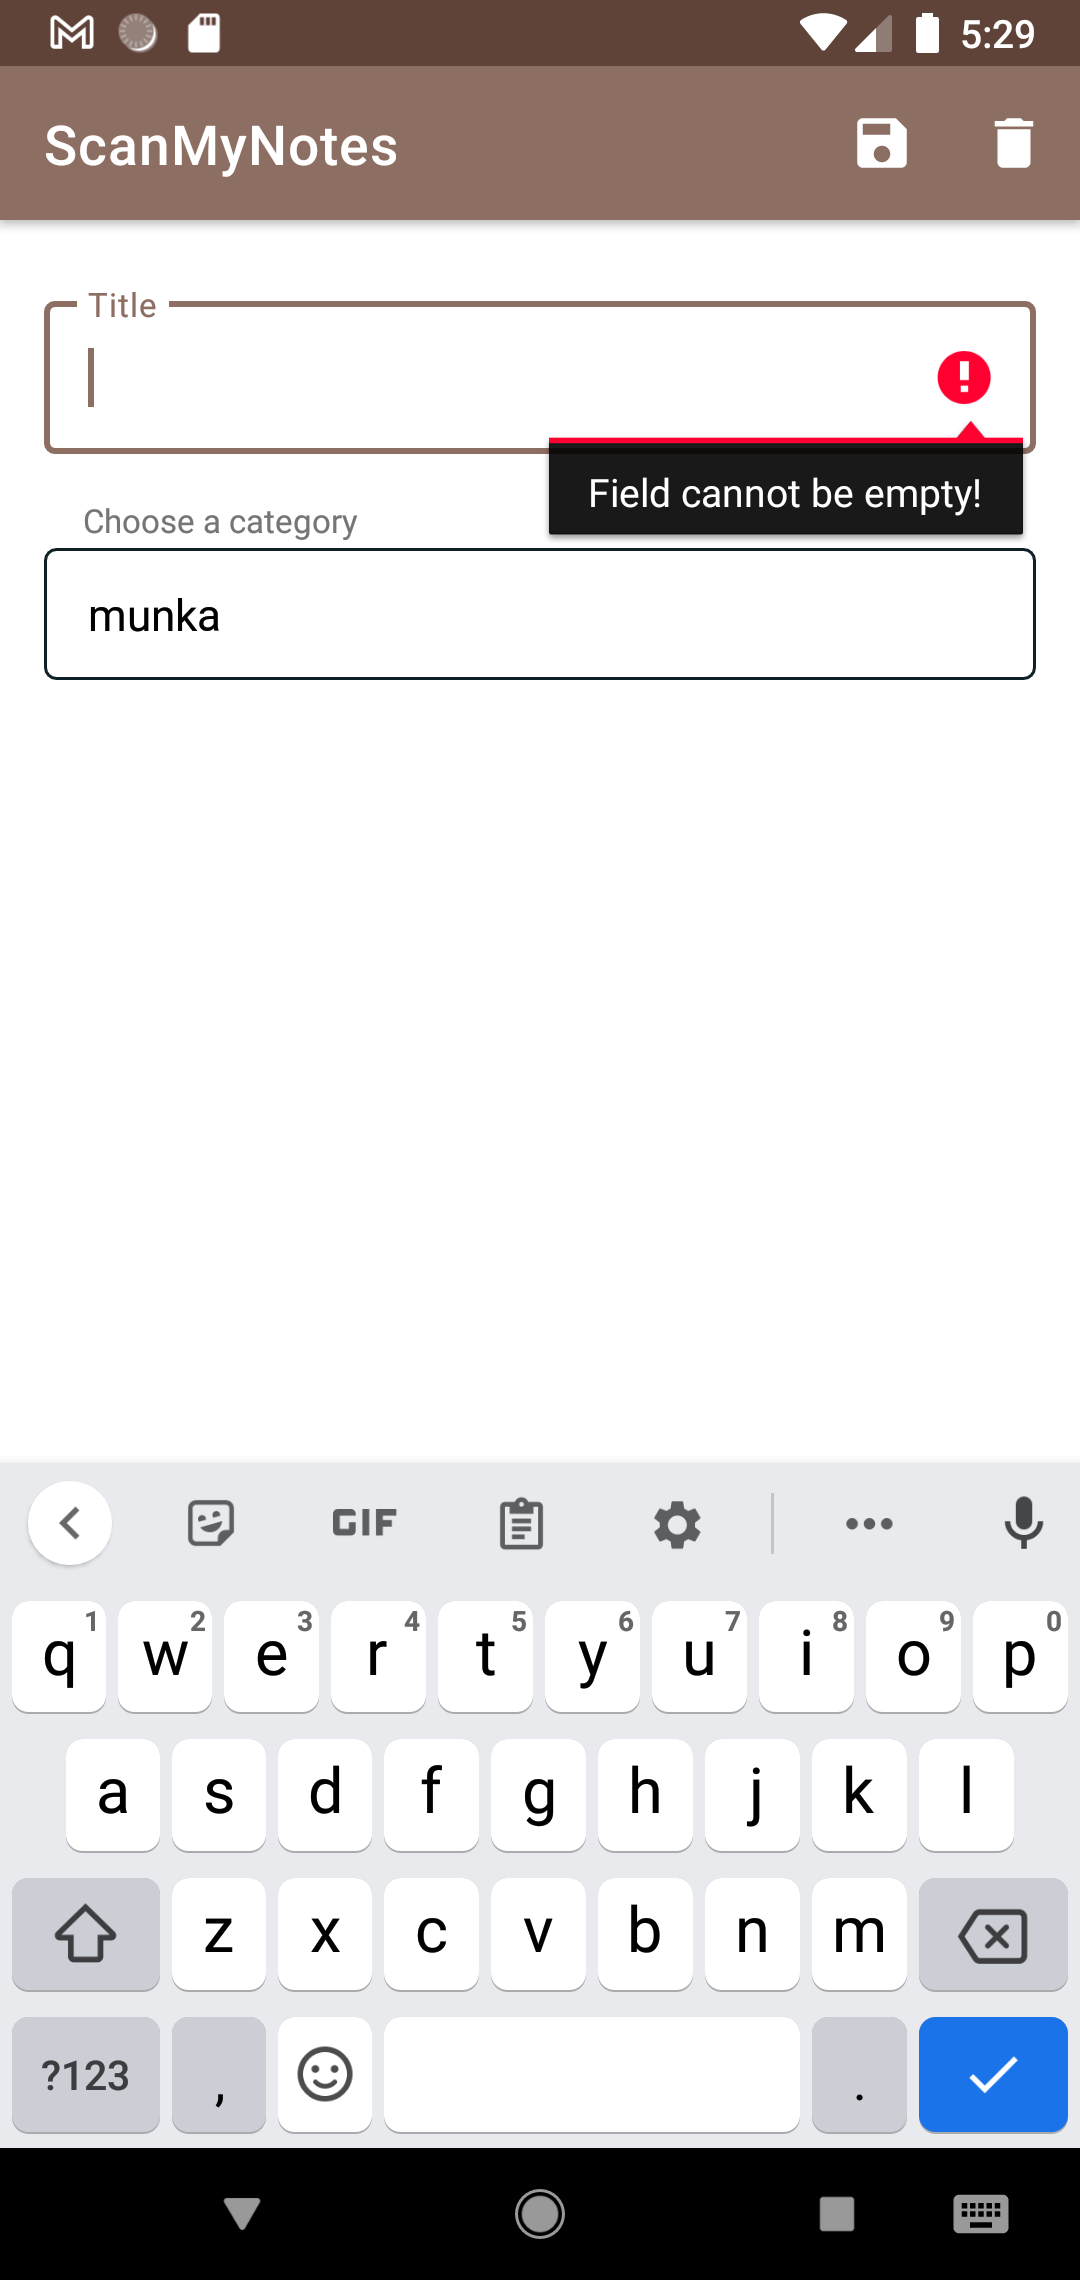
\includegraphics[width=50mm, keepaspectratio]{figures/category_edit_error.png}
	\caption{A kategória részletes képernyője, illetve a szerkesztési képernyő által feldobott hiba, ha üresen hagyjuk a címet.}
	\label{fig:CategoryDetailsScreen}
\end{figure}

\section{Megvalósítás}

A következőkben az alkalmazás implementációjába fogok részletesebben belemenni a projektfelépítéstől kezdve a logikán át a felhasználói felületig.

\subsection{Projektfelépítés}
A projekt elrendezése úgy lett kialakítva, hogy megfeleljen az Android fejlesztéshez ajánlott konvencióknak, emellett a package-ek nevei egyértelműek legyenek és könnyedén meg lehessen találni bármit, amit keresünk. A felépítés a következő:
\begin{itemize}
	\item \emph{data:} Az adatelérési réteg osztályait tartalmazza. Két package található benne: egy \emph{models} és egy \emph{network}. Előbbi a hálózati modell(eke)t tartalmazza, utóbbi pedig az API-kat és a DataSource-okat.
	\item \emph{di:} Az architektúra ajánlása alapján ebbe a package-be kell tenni a függőséginjektálás működéséhez szükséges fájlokat.
	\item \emph{domain:} A domain réteg tartalmazza az üzleti logikát. Ez általában interactorokból és üzleti modellekből áll. Jelen applikációban az egy darab interactort és a modelleket jelenti.
	\item \emph{ui:} Ez tartalmazza a felhasználói felülethez kapcsolódó összes kódot, azaz itt találhatók a Fragmentek, ViewModelek, ViewState-ek, illetve egyéb, megjelenítéshez kapcsolódó szükséges osztályok.
	\item \emph{util:} Ide kerültek azok a kódok, amiket máshova nem lehetett beilleszteni. Egyetlen fájl található benne, olyan kiegészítésekkel, amiket több osztály is használ, ezért nem lehetett egy funkcióhoz kötni.
\end{itemize}

\subsection{Szerveroldali komponensek integrációja}
Az alkalmazás backendjét a Firebase szolgáltatja, melynek kiterjedt és alapos dokumentációja nagyban megkönnyíti az integrációs folyamatot.

Első lépésként be kell jelentkezni a Firebase console\footnote{\url{https://console.firebase.google.com/}}-ba, és létrehozni az alkalmazás számára egy Firebase projektet. Amikor kész, akkor ehhez hozzá kell adni a már létező applikációt azáltal, hogy megadjuk az alkalmazás package nevét\footnote{A package név egy egyedi azonosító, mely alapján egyértelműen meghatározható az alkalmazás. Két ugyanolyan package névvel rendelkező applikáció nem telepíthető fel egy eszközre, de még a Google Play Store-ba sem kerülhet.}. Ezután generálódik egy \emph{google-services.json} nevű fájl, melyet le kell tölteni, és a lokális projekt \emph{app} mappájába beilleszteni. A projekt szintű \emph{build.gradle} fájlba fel kell venni a Google Services Gradle plugint, mint függőséget, és ezt a modul szintű \emph{build.gradle} fájlban egy \emph{apply plugin} parancs felvételével alkalmazni kell. Végül pedig a használni kívánt Firebase szolgáltatásokat is fel kell venni függőségként az utóbbi fájlba, és egy gradle szinkronizálás után elérhetővé válnak az alkalmazásban.

A projektben négy Firebase szolgáltatás került felhasználásra, melyek az Authentication, Firestore, Analytics és Crashlytics. Az alkalmazásban használt kódon kívül a menedzselésük a fentebb említett console-ban lehetséges, mely rendkívül kényelmes. Minden modul külön-külön be- és kikapcsolható a projekt igényeinek megfelelően, így az alkalmazás növekedésével később akár plusz funkciókat is bevezethetünk, mindössze egy kattintással.

Az első szolgáltatás az Authentication, mely elég fontos aspektusa a működésnek. Bekapcsolás után számos lehetőség tárul elénk, de teljes mértékben miénk az irányítás: alapértelmezetten minden ki van kapcsolva, csak azt fogjuk tudni használni, amit mi magunk kapcsolunk be. A \emph{Sign-in method} fülre kattintva tudunk egy vagy több bejelentkezési módot választani, melyet az alkalmazásban használni szeretnénk. Támogatja az autentikációt e-mail és jelszó, telefonszám, Facebook, Google, Apple és GitHub használatával, és ezeken kívül még néhány módszerrel. A projektben az e-mail és jelszó kombinációját választottam, ugyanis ahhoz vannak a legjobban hozzászokva a felhasználók, az e-mail cím az, ami tényleg mindenkinek van, ellentétben egy Apple vagy egy Google fiókkal. Legalább egy bejelentkezési módot bekapcsolva pedig a \emph{Users} fülön láthatjuk a regisztrált felhasználók listáját (\refstruc{fig:AuthUsers})

\begin{figure}[!ht]
	\centering
	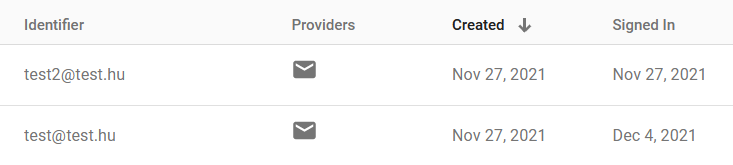
\includegraphics[width=120mm, keepaspectratio]{figures/auth_users.png}
	\caption{A regisztrált felhasználók listája.}
	\label{fig:AuthUsers}
\end{figure}

A bejelentkeztetést a \emph{ui.login} package-ben található \emph{LoginFragment} végzi. Ő a többi képernyővel ellentétben csak egy sima Fragment, nem a RainbowCake architektúra része, ugyanis tulajdonképpen két függvényből áll az egész, így nem tartottam célszerűnek végigvezetni a rétegeken. Ahogy azt a \refstruc{fig:MaterialBeforeAfter} korábban bemutatta, egyetlen képernyő áll rendelkezésre mind a bejelentkezéshez, mind a regisztrációhoz. Ez a döntés azért született meg, mert az alkalmazás jelenlegi funkcionalitásában nincs szerepe a felhasználói profilnak, nincs szükség semmilyen plusz információra a felhasználótól, ami később bármilyen formában felhasználásra kerülne, így felesleges két teljesen ugyanolyan UI-t készíteni csak a megkülönböztetés kedvéért.

Az autentikáció végrehajtásához a Firebase biztosít egy \emph{FirebaseAuth} típusú objektumot, melyen keresztül elérhető az összes ezzel kapcsolatos művelet. Meg lehet nézni, hogy van-e bejelentkezett felhasználó, és ezzel átugorható a bejelentkezési folyamat, ha valaki korábban már használta az alkalmazást. Ha nem, akkor pedig (e-mail és jelszavas bejelentkezés esetén) a \emph{signInWithEmailAndPassword} és a \emph{createUserWithEmailAndPassword} függvények állnak rendelkezésre, melyeknek az e-mail címet és a jelszót paraméterként megadva elvégzik a megfelelő műveletet. Az eredményt aszinkron módon küldi, amire egy \emph{onCompleteListener} segítségével lehet feliratkozni. Ezen belül ellenőrizhető a hívás kimenetele, és sikeres művelet esetén át tudunk navigálni az alkalmazás megfelelő képernyőjére, hiba esetén pedig kezelni tudjuk azt.

A következő szolgáltatás a Firestore, mely adatok felhőalapú tárolását teszi lehetővé egy hierarchikus struktúrában. Bekapcsolása után elérhetővé válik a kezelőfelülete, ahol szabályokat adhatunk meg a hozzáférésre, illetve láthatunk minden tárolt adatot egy könnyen átlátható vizuális reprezentációban. Az alkalmazás adatai az (\refstruc{fig:Firestore}) által mutatott módon kerülnek tárolásra.

Az összes adat egy \emph{users} nevű kollekcióban található, amiben minden felhasználóhoz tartozik egy dokumentum, melynek neve a regisztrációkor generált UID. Mivel ez garantáltan egyéni, így mindenki csak a saját adatait fogja elérni, és nem fordulhat elő, hogy egy felhasználó tudtán kívül felülírja egy másik adatait. A felhasználók dokumentumai két kollekciót tárolnak: egyet a kategóriáknak, és egyet a jegyzeteknek. Ezeken belül egy-egy dokumentum tárol egy-egy jegyzetet illetve kategóriát, melyeknek szintén egyéni azonosítója van.

Az alkalmazásban a \emph{data.network} package-ben található \emph{FirebaseApi} nevű osztály végzi az adatok lekérését és objektumokká való konvertálását. Az adatbázist egy \emph{FirebaseFirestore} típusú objektumon keresztül érem el, a \refstruc{fig:FirestoreQuery} által mutatott kóddal.

\begin{figure}[!ht]
	\centering
	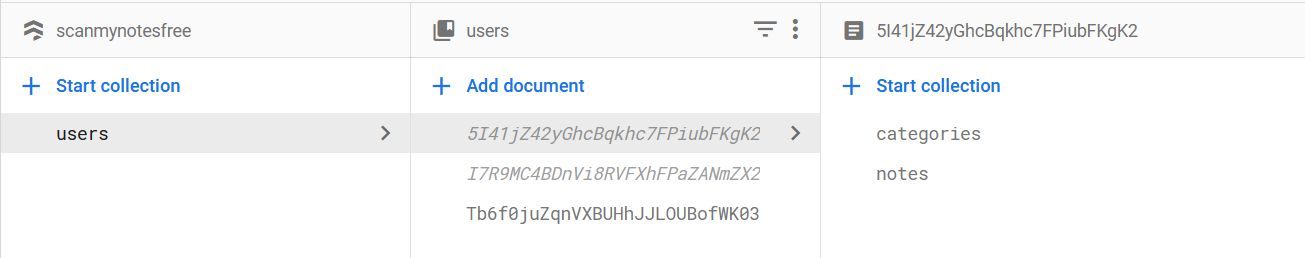
\includegraphics[width=150mm, keepaspectratio]{figures/firestore.png}
	\caption{A felhasználók adatainak struktúrája.}
	\label{fig:Firestore}
\end{figure}

\begin{figure}[!ht]
	\centering
	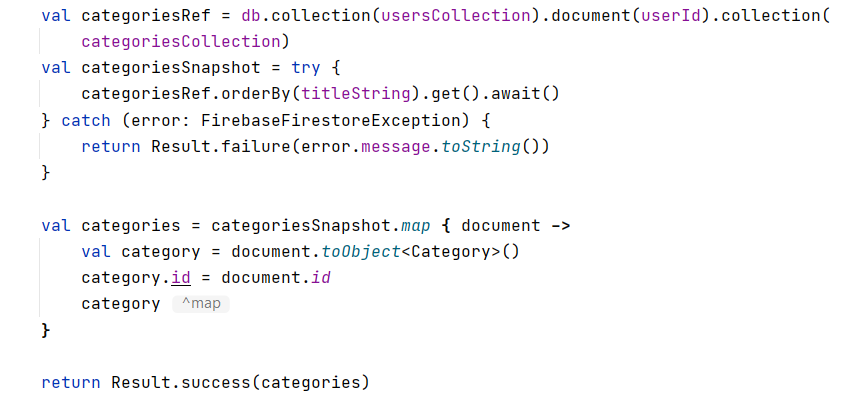
\includegraphics[width=150mm, keepaspectratio]{figures/firestore_query.png}
	\caption{A kategóriák lekérésének kódja az adatbázisból.}
	\label{fig:FirestoreQuery}
\end{figure}

Itt a \emph{db} változó az a bizonyos objektum, melyen keresztül elérhető az adatbázis. A hívástól függően egy \emph{CollectionReference} vagy egy \emph{DocumentReference} lehet az eredmény, ami az adott kollekció/dokumentum helyére mutat. Ezek felhasználhatók adatok írására és olvasására, ha pedig nem létezik adat azon a helyen, akkor létrehozza azt. Alapértelmezetten a referenciákon végzett minden hívás aszinkron módon hajtódik végre, de ez a működés nem volt ideális az alkalmazásom számára, ezért a \emph{kotlinx.coroutines.tasks.await()} függvény segítségével bevárom a lekérdezés eredményét. Ezután már csak annyi van hátra, hogy a visszakapott Snapshot objektumból kialakítsam azokat a típusokat, amikre szüksége van az alkalmazásnak. Szerencsére ez rendkívül egyszerű, mivel a Firestore biztosít egy \emph{toObject} függvényt, melynek a kívánt típust template-paraméterként megadva elvégzi a konverziót. Az id-t pedig azért kell még utána beállítani a kapott objektumon, mert az nem egy tárolt mezője a dokumentumnak, hanem az azonosítója, így arra nem terjed ki a \emph{toObject}.

A harmadik szolgáltatás az Analytics, mely rengeteg hasznos információt szolgáltat a felhasználókról és szokásaikról. Az előzőekhez hasonlóan itt is egy objektum biztosítja a kívánt funkcionalitást, melynek típusa ez esetben \emph{FirebaseAnalytics}. Ez figyel pár darab beépített eseményt, mint például a képernyők látogatását vagy a munkamenet-kezdést, de sajátot is lehet definiálni (\refstruc{fig:Analytics}). Itt egy új felhasználó regisztrációját rögzíti a rendszer annak metódusával együtt, ami jelen esetben e-mail és jelszó.

\begin{figure}[!ht]
	\centering
	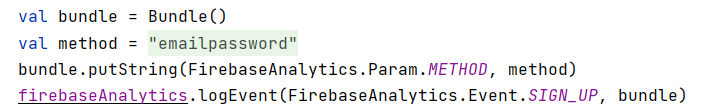
\includegraphics[width=120mm, keepaspectratio]{figures/analytics_custom.png}
	\caption{Egyéni esemény létrehozása és logolása Analytics segítségével.}
	\label{fig:Analytics}
\end{figure}

Az utolsó Firebase szolgáltatás, amit az alkalmazásban felhasználtam, a Crashlytics. Az előzőektől ellentétben az első bekezdésben leírtakon kívül ennél még szükség van további integrációs lépésekre is a működéshez. Van ugyanis egy saját pluginja, amit a fentiekkel megegyező módon fel kell venni mindkét gradle fájlba. Ezt követően szükség van egy teszt crash előidézésére, majd az alkalmazás újraindítására, hogy az elküldhesse a hibajelentést a Crashlyticsnek. Ezt követően viszont nincs már szükség semmi másra, a kódba sem szükséges semmit felvenni, mert automatikusan figyeli az alkalmazást. Természetesen számos lehetőségünk van finomhangolni a működését egyéni kulcsok hozzáadásával, de akár a nem-végzetes hibák figyelésével is.

\subsection{Képfeldolgozás integrációja}
Az alkalmazás fő funkciója a kézírás-digitalizálás, amit a Google Cloud Vision API végez. Ennek az ökoszisztémája nagyon hasonló a Firebase-hez, annyi különbséggel, hogy itt a Google Cloud Console\footnote{\url{https://console.cloud.google.com/}}-ban kell létrehozni a projektet. Ezt a kettőt akár össze is lehetne kötni, lévén Google rendszer mindkettő, de akkor a Firebase szolgáltatások is átkerülnek ingyenesről egy úgynevezett \emph{pay as you go}\footnote{A pay as you go olyan fizetési opció, mely során egy bizonyos kvóta alatt ingyenesen használhatók a szolgáltatások, afölött pedig annyit kell fizetni, amennyit használjuk.} plan-re. Én pedig szerettem volna minimalizálni az esetleges költségeket, így elvetettem ezt a lehetőséget.
	
Miután ez kész, célszerű a számlázás bekapcsolásával és egy \emph{billing account} létrehozásával kezdeni, mert bár mindent be lehet állítani enélkül is, addig nem fog működni az alkalmazásban az API, ameddig ez nincs rendben.

A következő lépés a kívánt API bekapcsolása, ugyanis itt is minden alapértelmezetten ki van kapcsolva. Ehhez az APIk közül kikerestem a Cloud Vision-t, majd egyetlen gombot kellett megnyomnom. A működéséhez azonban ennyi még nem elég, mert a használatához autentikálni is kell a kliensalkalmazást. Ehhez én egy API kulcsot hoztam létre, és létrehoztam egy apikey.properties nevű fájlt, melybe felvettem. Ezt úgy lehet felhasználni a projektben, hogy a \refstruc{fig:ApiKey} és a \refstruc{fig:ApiKeyConfig} kódrészleteit fel kell venni a modul szintű \emph{build.gradle} fájlba. A második ábrán látható, ahogy egy \emph{string} típusú és \emph{VISION\_API\_KEY} nevű változót csinálunk a fájlból kiolvasott kulcsból. Mindez azért szükséges, mert az API kulcs egy érzékeny adat, annak segítségével bárki felhasználhatja a saját alkalmazásában a szolgáltatást az én nevem alatt. Tekintve pedig, hogy fizetős szolgáltatásról van szó, ezt még komolyabban védeni kell, hogy ne szenvedjek anyagi kárt. Ezzel a módszerrel pedig rendkívül egyszerű ezt megtenni, hiszen a verziókezelő rendszerbe való feltöltés előtt csak annyit kell tenni, hogy az apikey.properties fájlt kivesszük a követés alól.

\begin{figure}[!ht]
	\centering
	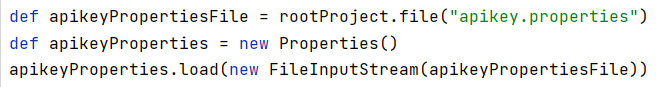
\includegraphics[width=120mm, keepaspectratio]{figures/gradle_apikey.png}
	\caption{A létrehozott apikey.properties fájl használata a projektben.}
	\label{fig:ApiKey}
\end{figure}

\begin{figure}[!ht]
	\centering
	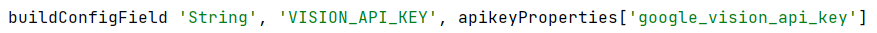
\includegraphics[width=150mm, keepaspectratio]{figures/apikey_configfield.png}
	\caption{A megfelelő API kulcs kiolvasása a fájlból.}
	\label{fig:ApiKeyConfig}
\end{figure}

A képfeldolgozás megvalósítása a következő: a fotózás befejezésével a kép egy Bitmap objektumként érkezik meg az interactorhoz, ahol a hívás háttérszálra kerül. Ezáltal már biztonságosan lehet hosszabb műveleteket végezni, így itt végzem el kép base64 kódolását, mely során egy Vision API által biztosított Image típusú objektumot állítok elő. A további hívások már ezt az objektumot kapják paraméterként, így a DataSource-on keresztül a \emph{VisionApi} osztályhoz jut. Ez végzi a további előkészítési folyamatot, küldi el detektálásra a képet, és az eredményt a megfelelő formában adja vissza. Mindez meglehetősen egyszerűen megoldható az API saját objektumainak használatával. Itt először megadom az API kulcsot, majd specifikálom a kívánt detektálási módot. Ez azért fontos, mert az API a kézírás-felismerésen kívül számtalan másra is képes, így nekem kell kiválasztanom, hogy pontosan mit szeretnék elvégeztetni. Ezután a képből és a választott funkcióból egy \emph{BatchAnnotateImageRequest} objektumot készítek (ami jelenleg egyetlen képet tartalmaz, de van lehetőség egyszerre több kép feldolgozására is), és az \emph{annotate} függvény segítségével megkapom ennek az annotációját. A teljes szöveget az eredmény \emph{fullTextAnnotation} tagváltozója tartalmazza.

\subsection{Adatmodellek elkészítése}
Az alkalmazásban szükség volt olyan osztályokra, melyek az adatbázisból visszakapott adatokat fogják össze, és szállítják a rétegek között. Ezeket hívják adatmodellnek, és a megvalósítás során négy darabot készítettem. Ebből három a \emph{domain.models} package-ben található, ezek egyben a megjelenítési modellek is, egy pedig a \emph{data.models} package-be tartozik, ugyanis hálózati hívások eredményét reprezentálja.

Ez utóbbi a Result nevű osztály, és tulajdonképpen a visszakapott adatokat vagy hibaüzenetet csomagolja be a könnyebb hibakezelés érdekében. Egy sablonosztályról\footnote{Olyan osztály, mely template paramétereket használ, ezáltal tetszőleges adattípussal használható.} van szó, mely két belső \emph{data class}-t tartalmaz: egy Success, illetve egy Failure nevűt. A Success a sikeres hívások eredményét tárolja egyetlen \emph{data} nevű paraméterében, mely tetszőleges adattípust felvehet, a Failure pedig a sikertelen hívások hibaüzenetét továbbítja. Emellett \emph{companion object}\footnote{Kotlinban a companion object tartalmazza tulajdonképpen azokat az adattagokat és függvényeket, amelyeket Javaban statikusnak hívtunk. Ezek osztályszintűek, ami annyit jelent, hogy nincs szükség az osztály példányosítására ahhoz, hogy elérjük őket.}-ben tartalmaz egy-egy függvényt, melyekkel a két állapot valamelyikét lehet inicializálni. A FirebaseApi összes függvényét úgy implementáltam, hogy valamilyen Result típust adjon vissza, így a fentebbi rétegekben minden esetet könnyedén le lehet kezelni.

A domain modellek közül az első és legalapvetőbb a ListItem osztály. Ő egy \emph{open class}, mivel Kotlinban csak akkor származtathatunk le egy osztályból egy másikat, hogyha a szülőt megjelöljük az \emph{open} kulcsszóval. A ListItemnek pedig pont ez a funkciója, hogy közös őst biztosítson a kategóriák és a jegyzetek számára, ami főleg a kategorizált lista építésénél fontos. Tartalmazza a két osztály közös adattagjait, melyek az \emph{id, title} és \emph{parentId} névre hallgatnak. Ezek közül az utolsónak lehet null az értéke, amennyiben az adott elemnek nincs szülője a listában.

Ennek leszármazottai a Note illetve a Category nevet kapták. Ők az alkalmazásban tárolt és megjelenített jegyzeteket, illetve kategóriákat reprezentálják. Ősükhöz képest egy-egy adattaggal bővültek, a Note \emph{content} adattagja a jegyzetek szövegét tárolja, míg a Category \emph{listItems} listájában a tartalmazott objektumai találhatók. Ez utóbbi nincs eltárolva az adatbázisban, hiszen könnyedén előállítható az adatok lekérdezése után a \emph{parentId} adattagok alapján.

\subsection{Egyedi FloatingActionButton}
Az új adatok fevételéhez szükség volt valamilyen gombra, aminek a megnyomásával a felhasználó a megfelelő oldalra navigálhat. Mivel ez egy elég fontos funkció, így célszerű kitüntetett helyre tenni az alkalmazásban, ahol a felhasználók azonnal láthatják. Az ilyen típusú gombok megvalósítására készült el a Material Components könyvtár FloatingActionButton névre keresztelt komponense. Ez egy általában a jobb alsó sarokban elhelyezkedő, tartalom felett megjelenő gomb, mely görgetéstől függetlenül a képernyőn marad, így biztosítva a folyamatos elérhetőséget.

Azonban funkcionalitás szempontjából a kategóriák és a jegyzetek létrehozásához nekem két ilyen gombra lett volna szükségem, ami viszont szembemegy a Material Design alapelveivel. Ezért döntöttem úgy, hogy ezt felhasználva megalkotom a gombot amire szükségem van (\refstruc{fig:FloatingActionButton}).

\begin{figure}[!ht]
	\centering
	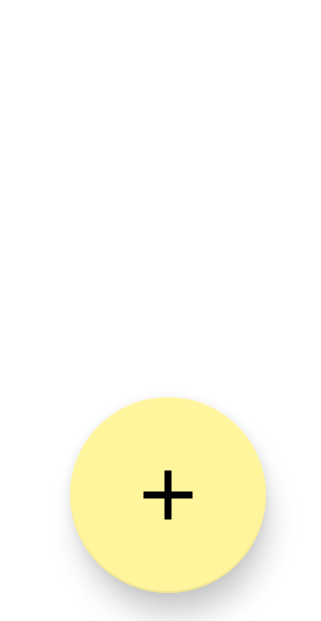
\includegraphics[width=30mm, keepaspectratio]{figures/floatingbutton_closed.png}
	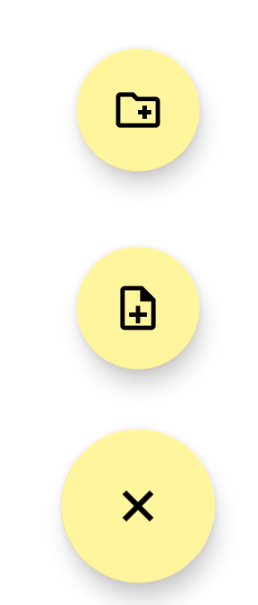
\includegraphics[width=32mm, keepaspectratio]{figures/floatingbutton_open_small.png}
	\caption{Az elkészített egyedi gomb alapértelmezett és kinyitott állapotban.}
	\label{fig:FloatingActionButton}
\end{figure}

Működése a következő: alapértelmezett állapotban a bal oldali ábrán megjelenő egyetlen gomb látszik. Erre kattintva egy animációval elfordul 45 fokkal, és közben a másik kettő, kicsit kisebb gomb alulról beúszik és fokozatosan megjelenik. A két újonnan megjelent gomb biztosítja a jegyzetek és kategóriák létrehozásának lehetőségét, az eredeti gombot megnyomva pedig a kezdeti állapot áll vissza.

Ehhez először is a listanézeten elhelyeztem három FloatingActionButtont a jobb alsó sarokba, egymás fölé. Létrehoztam három erőforrásfájlt az ikonoknak, a legalsó egy pluszjelet kapott, a felette lévő egy új jegyzet ikont, a felső pedig egy új mappa ikont. A felső kettő alapértelmezett láthatóságát \emph{gone}-ra állítottam, ami a helyes működéshez elengedhetetlen, ugyanis ha csak \emph{invisible} állapotban van egy UI elem, akkor ott marad a képernyőn, csak látszani nem fog, ami ezen gombok esetében azt eredményezné, hogy a mögötte lévő terület nem lenne kattintható.

Ezután következtek az animációk, melyeket Androidon szintén erőforrásfájlokkal lehet megoldani XML-ben. A projektben ezeket a \emph{res/anim} mappába kell elhelyezni, és a kívánt hatás eléréséhez négy darabra volt szükségem. Egy ilyen XML fájl gyökér eleme egy set, melyben egy UI elem pozícióját, méretét, elforgatását és átlátszóságát animálhatjuk. Az alábbi képen a gomb kinyitási animációjának kódja látható (\refstruc{fig:ButtonAnimation}).

\begin{figure}[!ht]
	\centering
	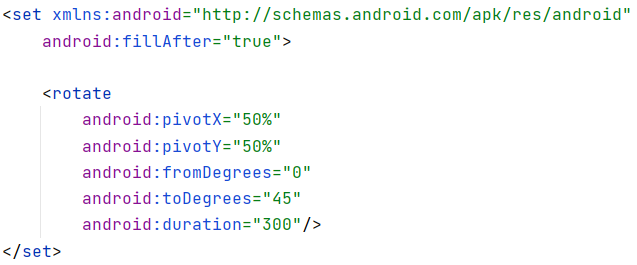
\includegraphics[width=110mm, keepaspectratio]{figures/animation_example.png}
	\caption{A kezdeti gomb elforgatásának animációja XML-ben.}
	\label{fig:ButtonAnimation}
\end{figure}

Ami a legérdekesebb, hogy a pivotX és pivotY tulajdonságokkal meghatározhatjuk, hogy az adott elem forgatásakor a középpont hol legyen. Így egészen komplex animációk is létrehozhatók, habár nekem most csak egy egyszerű középpont körüli forgatás kellett.

\subsection{Egyedi legördülő menü}
Létrehozás és módosítás során lehetőséget ad az alkalmazás kiválasztani egy kategóriát, melybe az objektumot tenni szeretnénk. Ennek megvalósítására a legördülő menüt találtam legalkalmasabbnak, melyet Androidon a \emph{Spinner} nevet kapta. Ezt a komponenst egy ArrayAdapter segítségével töltöm fel, mely a neki odaadott kollekció minden elemére visszaad egy, a létrehozásakor megadott layout-ot, ami itt most egy alapértelmezett \emph{simple\_spinner\_dropdown\_item}. Ez remekül biztosítja a számomra szükséges funkciót, csak épp nem túl esztétikus, és semmiképp sem illik a Material elemek közé. Ennek a megoldására két lehetőségem volt: a Material könyvtár részeként érkező TextField használata, vagy saját magam próbálok egy hasonló kinézetet elérni a Spinner testreszabásával. Az előbbi megoldás nagyon jól passzolt volna az alkalmazásba, de az egész logikát a Spinner-re építve írtam meg, és sajnos a TextField használata ettől teljesen eltér, úgyhogy mindent át kellett volna írnom. Ezért az utóbbi opciónál döntöttem.

Ehhez kettő XML fájlt hoztam létre a \emph{res/drawable} mappában, egyet az inaktív, csukott állapot, és egyet a kinyitott állapot hátterének. Itt a \emph{shape} XML-attribútum segítségével tudunk különféle alakzatokat kirajzolni, alapértelmezettként pedig téglalapot rajzol. Nekem pont erre volt szükségem, így csak egy kicsit testre kellett szabni. Az inaktív háttér keretének adtam lekerekített sarkokat, paddinget és vonalvastagságot, emellett a színét beállítottam a Material TextField inaktív színére, hogy a lehető legjobban egyezzen a többi elem megjelenésével. A lenyitott háttér ettől annyiban különbözik, hogy a keret színe az alkalmazás fő színét kapta meg, dupla olyan vastag lett, és az egész kapott egy fehér kitöltést, hogy eltakarja a mögötte lévő elemeket. 

Ezekkel pedig úgy tudtam felülírni a Spinner eredeti kinézetét, hogy az XML-ben ráraktam az \emph{android:background} és \emph{android:popupBackground} attribútumokat, melyeknek értékül adtam a fent leírt két layout-ot. Így már egészen esztétikusra sikerült, és majdnem észrevehetetlen a különbség a többi elemhez képest. Az eredményt a \refstruc{fig:CustomSpinner} szemlélteti.

\begin{figure}[!ht]
	\centering
	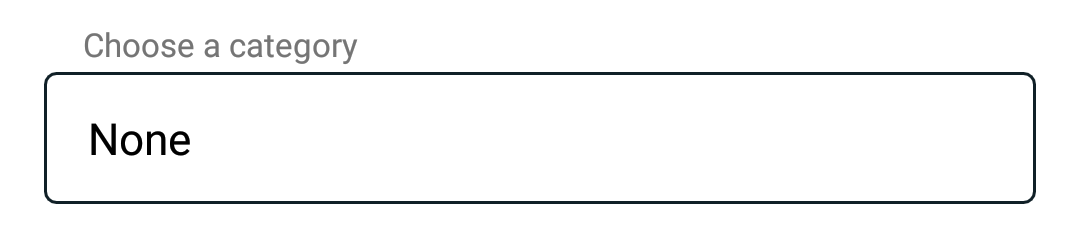
\includegraphics[width=65mm, keepaspectratio]{figures/custom_spinner_closed.png}
	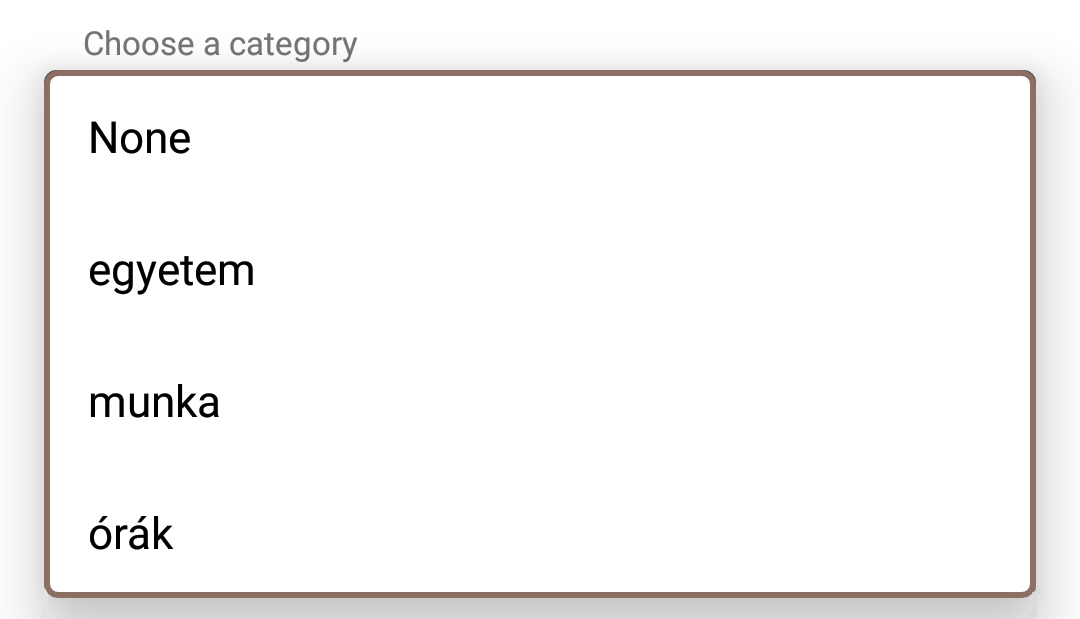
\includegraphics[width=65mm, keepaspectratio]{figures/custom_spinner_open.png}
	\caption{A Spinner kinézete becsukva, illetve kinyitva.}
	\label{fig:CustomSpinner}
\end{figure}

\subsection{Képernyők felépítése}
Habár a legtöbb felület elrendezése és funkciója eltérő, a felszín alatt hasonlóképpen működnek. Az alkalmazás a \emph{single activity}\footnote{Évekkel ezelőtt Android fejlesztés során az Activity szinonimája volt a képernyőnek, azaz minden megjelenő felülethez egy-egy Activity tartozott. Ám később a Fragmentek megjelenésével ez megváltozott, és most már a legelterjedtebb módszer a single activity alkalmazások fejlesztése, ahol egyetlen Activityből áll a program, és abban cserélődnek a Fragmentek.} struktúrát követi, így minden képernyő egy Fragment, melyhez a RainbowCake követelményei szerint tartozik saját ViewState és ViewModel. 

Egy ViewState itt nézettől függően három vagy négy állapotot tartalmaz. Mindegyik rendelkezik egy \emph{Loading} és egy \emph{Error} állapottal, melyek nevükhöz hűen a töltést, illetve valamilyen hibát jeleznek. Ezen kívül általában egy harmadik állapot jelzi az adatok helyes megérkezését, amikor a töltés befejeződött és megjeleníthető a UI, illetve a részletező nézetek logikája tér el ettől egy kicsit, mert ott a \emph{Viewing} és az \emph{Editing} állapotokkal lehet váltani az olvasási és az írási nézet között. 

A ViewModel-eknek minden esetben meg kell adni egy kezdő állapotot, ez mindegyik képernyőnél a \emph{Loading}. Emellett rendelkeznek egy \emph{load} függvénnyel, mely a kezdeti, megjelenítéshez szükséges adatokat kéri le, majd a hívás eredménye alapján állítja megfelelő állapotba a UI-t. Itt van nagyon nagy szerepe a létrehozott Result osztálynak, mert a visszakapott eredményt típus alapján szét lehet bontani, nem kell belenézni az adatba, hogy érvényes-e. Ahogy az már korábban említésre került, a ViewModel végez minden logikát, ami a képernyőhöz kötődik, hogy a Fragment-nek tényleg csak a UI megjelenítésével kelljen foglalkoznia. Ez szűri a listát kereséskor, elvégzi a rendezést, és függvényeket tartalmaz minden módosítási és létrehozási műveletre, amikkel továbbhív az interactor felé. Általában a kategória vagy jegyzet létrehozásának és törlésének eredményét egy eseményben továbbítja a Fragment-nek, ugyanis ilyenkor navigálni kell másik képernyőre. 

A Fragment kezel mindent, ami a látható felhasználói felülettel kapcsolatos, hiszen csak neki van referenciája az elrendezésre és a benne található elemekre. Ez a referencia egy úgynevezett \emph{ViewBinding} funkció segítségével jön létre, melyet a \emph{build.gradle}-ben bekapcsolva minden layout-ot tartalmazó XML fájlhoz generálódik egy Binding osztály, melynek egy példányán keresztül közvetlenül elérhetjük az elemeit. Ezek a layout-ok mind ViewFlipper-t használnak, hogy a lehető legkönnyebb legyen cserélni a megjelenített nézetet (\refstruc{fig:ViewFlipperComponent}). A már korábban is szereplő ábrán látott layout gyerekeire a megjelenésük sorrendjének indexével lehet hivatkozni, azaz ebben az esetben a \emph{loadingView} a nullás, a \emph{noteListView} az egyes indexet kapja. Ám az ilyen számkonstansok hosszú távon nem eredményezik a legolvashatóbb kódot, ezért készítettem hozzá egy megfeleltetést, hogy a kódban a nevükkel hivatkozhassam őket (\refstruc{fig:ViewFlipperObject}).

\begin{figure}[!ht]
	\centering
	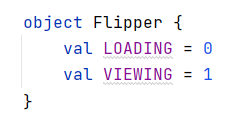
\includegraphics[width=50mm, keepaspectratio]{figures/viewflipper_object.png}
	\caption{A kezdeti gomb elforgatásának animációja XML-ben.}
	\label{fig:ViewFlipperObject}
\end{figure}

A ViewModel fentebb említett \emph{load} függvényét a Fragment az \emph{onStart} életciklus-függvényben hívja meg, mely minden alkalommal lefut, amikor a nézet láthatóvá válik. Azért ide tettem a hívást, mert az adatok frissítésére nem csak az első alkalommal van szükség, amikor megjelenik a Fragment, hanem minden módosítás után is, és erre ezt a megoldást láttam a legcélszerűbbnek. Az adatok frissítése után változni fog a képernyő állapota, melyet a \emph{render} függvényben tudunk lekezelni. Erre egy példa már szerepelt korábban az architektúra leírásánál, a \refstruc{fig:ViewFlipperUsage} bemutatásában.

\subsection{Kategorizált listanézet}
Az alkalmazás elindításakor megjelenő egymásba ágyazott lista a legbonyolultabb képernyő a projektben. Szükség volt hozzá egy RecyclerView-ra, mellyel egy listát jeleníthetünk meg a képernyőn, illetve a Groupie könyvtárra, amit már korábban bemutattam, de most az implementációs részleteibe fogok belemenni. 

Ahogy az a működésnél a képernyőképeken látszott (\refstruc{fig:NoteListScreen}), a kétféle listanézet között egy BottomNavigationView segítségével válthatunk. Az aktuálisan kiválasztott elem követésére létrehoztam egy SelectedNavItem nevű enumerációt, mely egy \emph{NOTES} és egy \emph{CATEGORIES} értéket tartalmaz. Ezáltal olvashatóan lehet kezelni a váltásokat, mindig egyértelmű lesz, hogy épp melyik képernyő van megjelenítve.

A folyamat a képernyők felépítésénél is leírt \emph{load} függvénnyel kezdődik, melynek itt egyetlen, az előző bekezdésben bemutatott SelectedNavItem típusú paramétere van. Szüksége van egy komplex, egymásba ágyazott listára, melyet az interactor \emph{getComplexList()} függvényének meghívásával kérhet le. Ez a hívás a NetworkDataSource-ban válik ketté, hiszen a FirebaseApi külön adja vissza a kategóriák, illetve a jegyzetek listáját. Miután a DataSource mindkét listát megkapja, összefésüli őket egy listába, mégpedig úgy, hogy abban csak azok az elemek szerepeljenek, amelyeknek nincs szülőkategóriája. Amelyik objektum \emph{parentId}-ja viszont tartalmaz értéket, annak megkeresi ezen id alapján a kategóriáját, és annak \emph{listItems} nevű adattagjához fűzi. Így pontosan egy olyan struktúrát kapok, mint amilyet meg szeretnék jeleníteni.

Ezt a listát először megkapja a ViewModel, majd a ListLoaded állapotba csomagolja, és megváltoztatja erre a viewState-et. Ezen változás hatására lefut a Fragment \emph{render} függvénye, melyben lecserélem a töltőképernyőt a listanézetre, a megkapott adatokat pedig átadom a lista adapterének.

A Groupie működéséhez két dolog kell: a listában tárolt elemek megvalósítása, illetve egy GroupieAdapter. Az elemek, melyek a \emph{notelist.items} package-ben találhatók, azért szükségesek, hogy a listában össze lehessen kötni az adatot az őt megjelenítő sorral. Két osztály készült ebből a célból, a CategoryItem és a NoteItem. 

A kettő közül a NoteItem az egyszerűbb, ez csak a Groupie által biztosított BindableItem osztályból származik le. Erre a ViewBinding használata miatt van szükség, és csak a három alap függvényt kell felüldefiniálni a működéshez: a \emph{getLayout}-ot, melyben specifikáljuk az egy sorhoz használni kívánt elrendezést, az \emph{initializeViewBinding}-ot, mellyel nevének megfelelően a ViewBindingot állítjuk be, hogy hozzáférjünk az elrendezés elemeihez, illetve a \emph{bind}-ot, melyben összekötjük a kettőt, és beállítjuk a megjelenítendő tartalmat. 

A CategoryItem valamivel bonyolultabb, hiszen ennél volt szükségem a kibontható és visszacsukható viselkedésre. Ezért ez a BindableItem-ből való leszármazáson kívül egy ExpandableItem nevű interfészt is megvalósít. Ez annyiban különbözik az alap item-től, hogy kell neki egy ExpandableGroup típusú tagváltozó, melyet a \emph{setExpandableGroup} függvényben a paraméterként kapott \emph{onToggleListener}-rel inicializálok. Ez biztosítja a kibontás/összecsukás működését és tárolja az aktuális állapotot, amit az \emph{isExpanded} tagváltozó segítségével lehet lekérni. 

A kategóriák sorának elrendezése annyiban különbözik a jegyzetektől, hogy a szövegen kívül egy nyíl ikont is tartalmaz, mely mindig jelzi, hogy az adott csoport éppen ki van-e bontva. Így a \emph{bind} függvény is változik annyiban, hogy a nyíl ikont is be kell állítani, illetve erre az ikonra tettem az \emph{onClickListener}-t, melynek hatására becsukódik/kinyílik a csoport és változik a nyíl iránya. 

Ezek után már csak az adapter maradt, mely a NoteListAdapter nevet kapta, és a GroupieAdapterből származik le. Ez tulajdonképpen egy wrapper osztály néhány funkcióval kiegészítve, hogy ne a Fragmentnek kelljen ezt a kódot tartalmaznia. Egy publikus függvénye van \emph{showList} néven, mely becsomagolja a lista kiürítését és feltöltését egy műveletbe. Először ugyanis hív az adapteren egy \emph{clear} függvényt - ami fontos, hiszen ha mindig csak hozzáadnánk, akkor folyamatosan sokszorozódna a megjelenített lista -, amit azért tettem bele ide, mert így nem kell külön a Fragmentben mindig meghívni, ezáltal kiküszöböl egy hibalehetőséget. Ezután a lista adapterhez adása előtt még meghívja az adatokon a privát \emph{populateList} függvényt, mely tovább hív egy rekurzív függvénybe, melynek kódja a képen látható (\refstruc{fig:PopulateList}).

\begin{figure}[!ht]
	\centering
	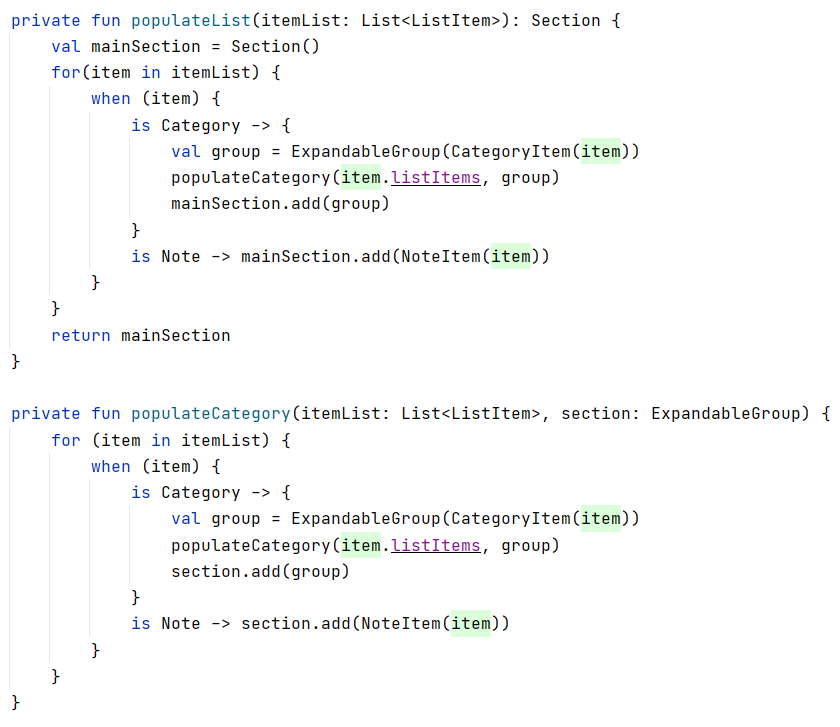
\includegraphics[width=145mm, keepaspectratio]{figures/list_population.png}
	\caption{Az adatok átalakítása megjeleníthető formátumba.}
	\label{fig:PopulateList}
\end{figure}

Ahogy látható, az adatok hierarchikus listáján megy végig, és a hierarchiát megtartva létrehoz egy immár NoteItemekből és CategoryItemekből álló listát. Erre a feladatra meglepően jól működik a rekurzió, hiszen sokkal könnyebb vele mélységi bejárást csinálni, a kívánt struktúrához ez pedig elengedhetetlen. 

Így a listakezelés a Fragmentben már rendkívül egyszerűvé válik, mert a NoteListAdaptert a RecyclerView adaptereként beállítva elég csak egy \emph{showList}-et hívni bárhol, ahol meg kell változtatni a megjelenített lista tartalmát. 

\subsection{Egyszerű listanézet}
Az egyszerű lista azt a nézetet jelenti, ami a BottomNavigationView \emph{Notes} elemére kattintva jelenik meg. Ez gyakorlatilag ugyanaz a képernyő, mint a komplex listáé, csupán a RecyclerView-ban lecserélődnek az elemek szimpla jegyzetekre. Emellett két funkció válik elérhetővé a listán, ami eddig el volt rejtve: a keresés és a rendezés. 

A keresésre kényelmes megoldást ad az androidx könyvtár SearchView komponense, mely egy előre elkészített, kattintható és gépelhető keresési nézet. Ám a működéséhez először még meg kell valósítani a \emph{SearchView.OnQueryTextListener} interfészt. Ez két felüldefiniálandó függvényt tartalmaz, melyekkel a keresés viselkedését lehet finomhangolni. 

Az első az \emph{onQueryTextSubmit}, ami akkor hívódik meg, amikor a felhasználó beírta amit szeretett volna, és a billentyűzeten megnyomja a kereséssé alakult enter gombot. 

A második pedig az \emph{onQueryTextChange}, mely minden alkalommal lefut, amikor változik a keresőmező tartalma. Én ez utóbbi használata mellett döntöttem, mert manapság a felhasználók nagy része elvárja az azonnali eredményt, amint leütik a billentyűt, és tagadhatatlanul kényelmes, hogyha már gépelés közben visszajelzést kapunk. Itt, amennyiben az új szöveg üres, azaz a felhasználó kitörölte a keresési mező tartalmát, akkor a teljes listát adja az adapternek, egyébként pedig a ViewModel végez egy szűrést a begépelt karaktersor alapján a jegyzetek címére, és csak azokat az elemeket teszi az adapterbe, melyekre illeszkedett a keresés.

A rendezés a UI-on a keresés mellett található, és az ikonjáról első pillantásra felismerhető. Ehhez szintén készítettem egy enumerációt a rendezési módok tárolására \emph{SortOptions} néven, mely egyelőre csak a cím alapján vett rendezést támogatja növekvő és csökkenő betűrendben, de lévén enumeráció, könnyedén bővíthető. 

A gomb megnyomására egy dialógusablak ugrik fel, melyben ki lehet választani a kívánt rendezést (\refstruc{fig:NoteListScreen2} - harmadik kép). Alapértelmezetten növekvő betűrendben található a lista, így ez az opció lesz kiválasztva felhasználói input előtt. 

Egy ilyen testre szabott dialógust a beépített DialogFragment osztály segítségével lehet létrehozni. A projektben kettő is található, az egyik a kategóriatörlés előtti figyelmeztető DeleteWarningDialog, illetve a rendezéskor megjelenő SortDialog. Most ez utóbbit fogom bemutatni, de a másik is nagyon hasonló megvalósítás szempontjából. 

A dialógus megvalósítását azzal kezdtem, hogy leszármaztattam a DialogFragment osztályból, és felüldefiniáltam az \emph{onCreateDialog} függvényét. Itt egy AlertDialog.Builder objektum segítségével tudtam felépíteni az általam elképzelt dialógust. Ennek számtalan függvénye van a különböző tulajdonságok beállítására, de ebben az esetben kettőre volt csupán szükségem. Az egyik a \emph{setTitle}, mellyel nevéhez hűen a dialógus címét lehet megadni, a másik pedig a \emph{setSingleChoiceItems}. Ez utóbbi az érdekesebb, ugyanis itt lehet a logika legnagyobb részét implementálni. 

Három paramétert vár, amiből az első egy stringek tömbje, ami az elemek megjelenítendő nevét tartalmazza. Ehhez létrehoztam egy \emph{sorting.xml} nevű erőforrásfájlt a \emph{res/values} mappában, melyben felvettem egy sortingOptions nevű tömböt. Ezt az erőforrást a beépített \emph{getStringArray} függvénnyel lehet átemelni kódba, amivel teljes értékű tömbbé válik, és ugyanúgy lehet használni, mint bármely másik változót. Ennek a módszernek az előnye, hogy nincs beégetett string a forráskódban, ami növeli a karbantarthatóságot. 

A második paraméter egy egész szám, mely azt mondja meg, hogy a megjelenéskor hanyadik opció legyen kiválasztva a sorban. 

A harmadik pedig egy DialogInterface.OnClickListener objektum, melyet esetünkben egy lambda függvénnyel meg tudunk adni (\refstruc{fig:DialogBuilder}). Ahhoz, hogy a kiválasztott objektumot kinyerjük, a \emph{selected} indexet kell felhasználni az enumeráció \emph{values}\footnote{A values függvény az enumeráció konstans értékeinek tömbjét adja vissza a deklaráció sorrendjében.} függvény által visszaadott értékein. Utána eltároljuk a kiválasztott indexet, hogy a következő megnyitáskor is megfelelő elem legyen kijelölve, majd a kinyert objektumot a parentFragmentManager\footnote{Ez egy olyan FragmentManager, melynek segítségével a jelenlegi fragment kommunikálhat a többivel, amennyiben ugyanahhoz az Activity-hez tartoznak.}-en keresztül beállítjuk a dialógus eredményét. Ezen kívül a végén még kell hívni egy \emph{dismiss}-t, ugyanis alapértelmezett esetben a single choice dialógusok csak gombnyomásra tűnnek el, itt pedig a kívánt működés az, hogy a rendezés kiválasztását ne kelljen gombnyomással megerősíteni.

\begin{figure}[!ht]
	\centering
	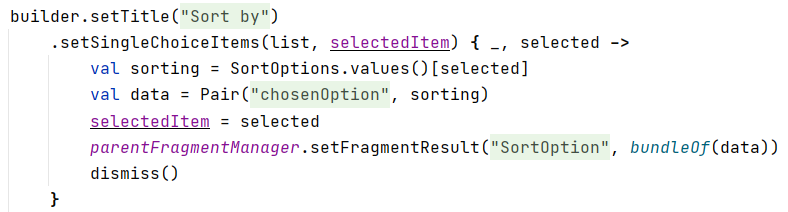
\includegraphics[width=140mm, keepaspectratio]{figures/dialog_builder.png}
	\caption{A dialógus beállításának kódja.}
	\label{fig:DialogBuilder}
\end{figure}

Ezután már csak annyi a teendő, hogy a Fragmentben, amiben kíváncsiak vagyunk a dialógus eredményére, fel kell iratkozni rá. Ezt a \emph{parentFragmentManager.setFragmentResultListener} függvénnyel tudjuk megtenni, aminek paraméterként meg kell adni azt a kulcsot, amilyen adatra kíváncsiak vagyunk. Ez a fenti képen a \emph{setFragmentResult} paramétere, melynek a SortOption nevet adtam. A kiválasztott rendezési módszer kinyerése után pedig a ViewModel által rendezett listát odaadjuk az adapternek megjelenítésre. 

\subsection{Navigáció}
A felhasznált könyvtáraknál már említésre került a Navigation Component, de itt most részletesen kifejtem a projektben betöltött szerepét. 

A megvalósítást azzal kezdtem, hogy felvettem a \emph{build.gradle} fájlba a könyvtárat függőségként. Ezután a MainActivity layout erőforrásába felvettem egy FragmentContainerView-t, és beállítottam, hogy ez töltse be az alapértelmezett NavHost szerepét. 

Ezt követően létre kellett hoznom a \emph{res/navigation} mappát, és abba felvenni egy navigációs gráfot. Ehhez tartozik egy kényelmes és intuitív grafikus felület (\refstruc{fig:NavGraph}), melyen könnyedén össze lehet rakni az appon belüli navigációt, de minden más erőforráshoz hasonlóan itt is fennáll a lehetőség, hogy kézzel XML-t írjunk. 

\begin{figure}[!ht]
	\centering
	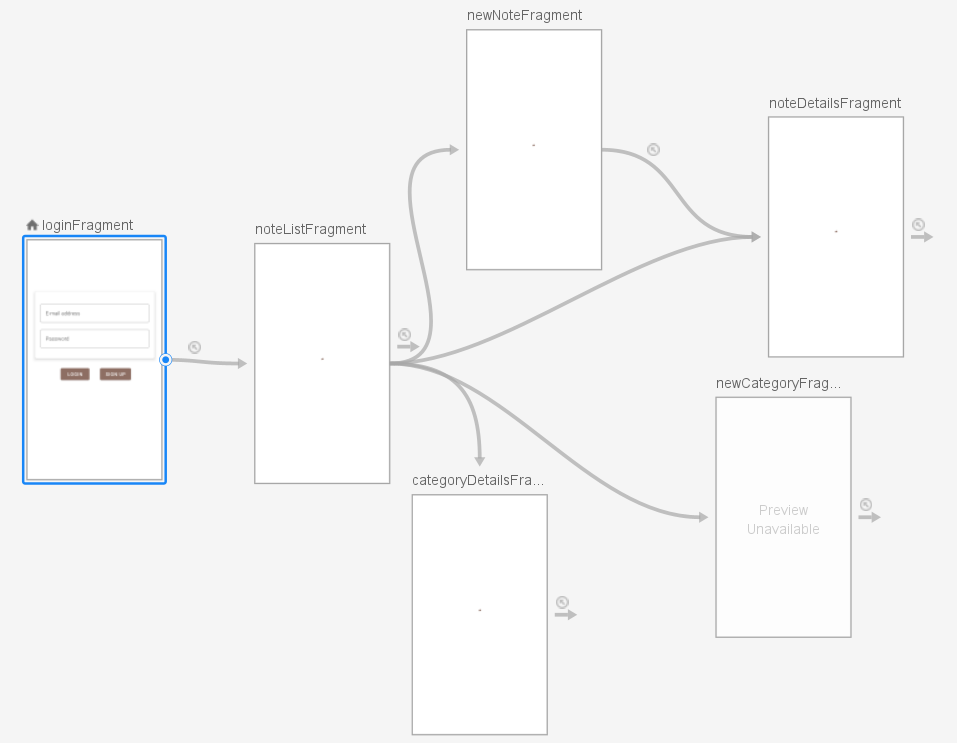
\includegraphics[width=150mm, keepaspectratio]{figures/nav_graph.png}
	\caption{Az alkalmazás navigációjának vizuális reprezentációja.}
	\label{fig:NavGraph}
\end{figure}

A felület oldalsó sávjaiból lehetőségünk van a kívánt fragmenteket behúzni a felületre, és különböző navigációs útvonalakat definiálni köztük. Ezeket az IDE akcióknak hívja, és sok információt tudnak tartalmazni. Azon kívül, hogy id-t és célt adhatunk egy akciónak, definiálhatunk navigáció közben megjelenítendő animációkat. Befolyásolni tudjuk a backstack állapotát, ami például bejelentkezés után rendkívül hasznos, hiszen szeretnénk elkerülni, hogy a felhasználó bejelentkezve a vissza gomb megnyomásával újra a bejelentkező oldalra kerüljön. Ezt egyszerű megoldani a Navigation Component segítségével, mert szimplán a felület popBehavior menüjében beállítjuk, hogy az adott akció elvégzésekor a kívánt fragmenteket levegye a backstackről, így visszafelé navigációkor nem fogjuk elérni. 

A másik nagyon hasznos funkció, ami megkönnyíti a fragmentek közti adatátadást, az az argumentum. Ezt szintén az akciókhoz tudjuk kötni, és a kiindulási fragmentben paraméterként megadni, így a célfragmentben elérhetővé válik az adat. Ennek kiegészítése a SafeArgs plugin, mely típusbiztos navigációt tesz lehetővé. Ez például a részletező nézeteknél nagyon hasznos volt, mert a listanézetben a kiválasztott elem id-ját át tudtam adni navigáció során a Details képernyőnek, annak pedig ezt elég volt átvennie, és a megfelelő id-val rendelkező objektumot lekérni az adatbázisból. 

Emellett még tartalmaz olyan könnyítést, hogy létre lehet hozni egy "visszatérő" akciót, mely automatikusan leszedi a backstackről saját magát, és úgy navigál vissza az őt megelőző fragmentre. Ez arra is nagyon jó, hogy ne legyen átláthatatlan a gráf, ugyanis ahogy az ábrán is látható, ezeket az akciókat úgy jelöli, hogy a fragmentből kifelé mutatnak, tulajdonképpen a "semmibe".

Ha a gráfon már szerepel minden, amire szükségünk van, akkor az egyetlen hátralévő dolog a kódból való használata. Ehhez először szükségünk lesz a NavController-re, amit a fragmentekből a \emph{findNavController} függvényhívással kaphatunk meg. Ezután kelleni fog az elvégezni kívánt akció. A SafeArgs-nak köszönhetően minden fragmenthez generálódik egy \emph{Directions} utótaggal ellátott osztály, mely tartalmazza a belőle kiinduló navigációs útvonalakat, olyan néven, amilyen id-t adtunk neki a gráfban. Így például a NoteListFragmentből kijelentkezni a \emph{NoteListFragmentDirections.logoutAction} felhasználásával tudunk. Így már nincs más hátra, mint a NavController \emph{navigate} függvényének paraméterként odaadni az akciót.

\subsection{Tesztelés}
Az alkalmazás fejlesztése során kétféle módon is ellenőriztem a helyes működést. Az első a manuális tesztelés, mely során mind emulátorban, mind fizikai készüléken végigmentem a funkciókon.

Fejlesztés közben számomra elengedhetetlen volt a manuális tesztelés, hiszen meglehetősen gyors visszajelzést ad a kódról, hogy megjelenik-e az új funkció, az elvárt módon jelenik-e meg és megfelelően működik-e. 

Az egész alkalmazás folyamatán végigmentem, az elejétől kezdve. Csak helyes formátumú e-mail címmel és legalább 6 karakter hosszúságú jelszóval lehet regisztrálni, ha ez nem teljesül, akkor a nem megfelelő tartalmú beviteli mező hibát dob. Nem létező felhasználóval vagy hibás adatokkal szintén nem lehet belépni. A kijelentkezés gomb is az elvárt módon működik, megnyomásával a felhasználó visszakerül a bejelentkezési oldalra. 

A kezdőoldalon kezdetben nincs tartalom, először létre kell hozni egy-két jegyzetet és kategóriát. Ehhez a jobb alsó sarok sárga gombja megfelelően működik, kattintásra az elvárt módon kinyílik és becsukódik, az animáció is működik. A felső gombra nyomva a kategória létrehozási képernyője jelenik meg, a szükséges két mezővel. A cím üresen hagyása hibát eredményez, a validáció helyesen működik. A Spinner-rel sincs probléma, a kiválasztott elem kerül elmentésre az új kategória szülőjeként. Létrehozás után a kezdeti listanézetre térünk vissza, az az elvártnak megfelelően frissül, és megjelenik benne az új elem. 

Kinyitott állapotban a középső gombra kattintva amennyiben nincs az alkalmazásnak engedélye a kamera használatára, akkor feljön egy rövid magyarázat, hogy miért van szükség az engedélyre. Itt az \emph{OK} gombra nyomva feljön a rendszer engedélykérése, melyet lehetősége van a felhasználónak elfogadni vagy elutasítani. Amennyiben elutasítja, akkor egy Toastot dob az alkalmazás, melyben leírja, hogy el kell fogadni a funkció használatához az engedélyt. Elfogadás után pedig megnyílik egy kamerafelület, ahol fényképet lehet készíteni. Ennek befejeztével rövid várakozás után az új jegyzet létrehozása képernyőre navigálunk, ahol a detektált szöveg megjelenik a tartalom mezőben. Itt lehetőségünk van módosítani rajta, illetve címet adni és szülőkategóriát választani. Itt a cím mellett a tartalomra is érvényes a megkötés, hogy nem lehet üres, addig nem fogjuk tudni elmenteni. 

Sikeres mentés után a jegyzet részletező nézetére kerülünk, ahol megfelelően megjelennek az adatai. A jobb felső sarokban a ceruza ikonra kattintva átvált szerkesztő nézetre, eltűnik a ceruza, és megjelenik egy pluszjel és egy mentés ikon. A pluszjelre nyomva újabb fényképet készíthetünk, és az abból visszaérkező szöveg hozzáfűződik az eddigi tartalomhoz. Itt a mentés ugyanúgy működik mint a létrehozásnál. Egy harmadik opció mind megtekintéskor, mind szerkesztéskor elérhető, és ez a törlés. Ennek hatására törlődik a jegyzet és visszanavigálunk a listanézetre, melyen frissülés után látható, hogy a kitörölt jegyzet eltűnt. 

A törlés a kategóriára is ugyanígy működik, annyi különbséggel, hogy előtte felugrik egy ablak, mely figyelmeztet, hogy ezzel minden gyerekét is elveszítjük. Ha itt meggondoljuk magunkat akkor nem történik semmi, de ha megerősítjük, akkor kitörlődik vele együtt az összes benne található jegyzet és kategória. Ilyenkor szintén a listanézetre navigálunk, és láthatjuk, hogy eltűnt. 

Még amit itt célszerű leellenőrizni, az az elemek áthelyezése egyik kategóriából a másikba. Ha belemegyünk a szerkesztésbe, és kiválasztunk egy másik szülőkategóriát az objektumnak, akkor mentés után a listában láthatjuk, hogy átkerült az újonnan beállított kategória alá. 

Miután a hierarchikus listanézet lehetőségeit kimerítettük, már csak a jegyzetek listájának ellenőrzése maradt. A BottomNavigationView-n a Notes elemet kiválasztva megerősíthetjük, hogy a lista megváltozik, és csak a jegyzetek kerülnek bele. A nézet tetején pedig megjelenik egy keresősáv és egy rendezés gomb.

A keresősáv aktiválódik ha belekattintunk, és gépelés közben folyamatosan szűri az eredményeket, törlés közben pedig egyre bővül az illeszkedő jegyzetek halmaza. Ha az utolsó betűt is kitöröljük a keresésből, akkor visszatér az eredeti, teljes lista. 

Ami a rendezést illeti, a gomb megnyomására az elvártnak megfelelően felugrik az ablak, alapértelmezetten az első opcióval kiválasztva. Ha kiválasztjuk a fordított betűrendet, akkor eltűnik a dialógus és újratöltődik a lista, megfelelően rendezve. Ha olyan opciót választunk, ami már aktív, akkor csak a dialógus tűnik el, de semmi nem történik, és ez így kell legyen, mert felesleges ugyanazt a listát újratölteni.

Ezután pedig következnek a unit tesztek. Ezekhez segítségül hívtam a JUnit 4 és Mockito könyvtárakat, melyek hatalmas segítségnek bizonyultak. Mindenképp szerettem volna legalább unit teszteket írni, mert előtte még sosem írtam, és szerettem volna megtanulni. Első körben a ViewModelek tesztelésére koncentráltam, mert az alkalmazásban azok végzik a legtöbb feladatot, főleg az ő munkájuk a lényeges. Nem készült még mindegyikhez teszt, és nem is teljes a lefedettség, de a célomat elértem: írtam unit teszteket és értem őket. 

A \emph{test/ui} mappába raktam őket, hiszen UI közeli logikáról van szó. A ViewModelekhez csináltam külön-külön tesztosztályokat, melyeken belül függvények ellenőrzik egy-egy funkció helyes működését. Ezek az osztályok a RainbowCake által biztosított ViewModelTest osztályból származnak le, melynek segítségével könnyedén meg lehet figyelni a teszt során előforduló állapotokat és eseményeket. 

Mivel a ViewModelek az Interactort hívják az adatok megszerzéséhez, ezért ezt minden ilyen osztályban mockolni kellett. Ebben segített a Mockito, mellyel a \emph{@Mock} annotációval megjelölt objektumoknak meg lehet szabni a viselkedését. Ehhez minden osztályban csináltam egy \emph{companion object}-et, mely tartalmazza az elvárt adatokat. Így a következőképp néz ki egy teszteset (\refstruc{fig:TestCase}).

\begin{figure}[!ht]
	\centering
	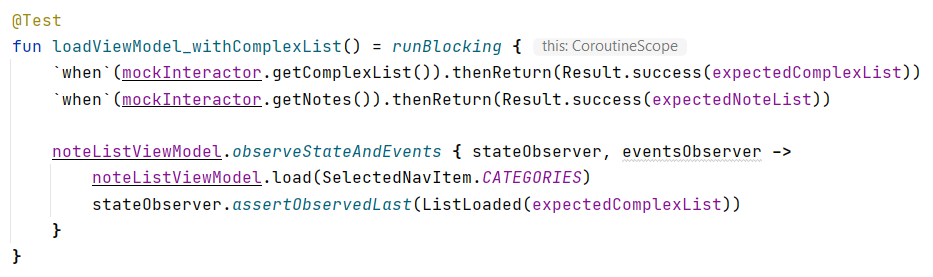
\includegraphics[width=150mm, keepaspectratio]{figures/test_case.png}
	\caption{A komplex lista unit tesztje.}
	\label{fig:TestCase}
\end{figure}

Ebből a lényeg szépen megfigyelhető: a \emph{when - thenReturn} függvénypárossal lehet megszabni a mock objektumok viselkedését. Ebben a tesztesetben sikeres esetet szeretnék tesztelni, úgyhogy mindkét interactor hívás sikerrel tér vissza. Ezután elkezdem a megfigyelést, majd elvégzem a tesztelni kívánt függvényhívást. Az adott observerek segítségével pedig validálom az elvárt állapotot. Ehhez azért használom az assertObservedLast függvényt, mert a sima assertObserved a futás során összes előforduló állapotot rögzíti, és nekem itt az a lényeg, hogy a hívás végére az elvárt eredményt kapjam, amihez elég a legutolsó megfigyelt állapot.